\documentclass[12pt]{article}

\usepackage{sbc-template}

\usepackage{graphicx,url}
\usepackage{tabularx}

\usepackage[brazil]{babel}   
\usepackage[utf8]{inputenc}

\usepackage{url}
\usepackage{hyperref}
\usepackage{placeins}

\sloppy

\title{Encontre na UFMS: facilitando a navegação pelo campus com cooperatividade}
\author{Filipe dos Santos Pires\inst{1}, Wilson Eduardo Fantucci Diniz de Almeida\inst{1},\\Ana Karina Dourado Salina de Oliveira\inst{1}}
\date{November 2024}
\address{Faculdade de Computação - Universidade Federal do Mato Grosso do Sul
  (UFMS)\\Campo Grande - MS - Brasil
  \email{filipe\_pires@ufms.br, wilson.eduardo@ufms.br, ana.salina@ufms.br}
}

\begin{document}

\maketitle

  \begin{resumo} 
    Este artigo descreve o desenvolvimento do aplicativo móvel ``Encontre na UFMS'', que surgiu devido a falta de acessibilidade de informações dos locais presentes no campus de Campo Grande da UFMS, para alunos, visitantes e docentes que fosse concentrados em uma aplicação. O principal objetivo do aplicativo Encontre na UFMS é oferecer uma ferramenta simples e acessível para ajudar os seus usuários a encontrarem pontos de interesse, além de possibilitar a cooperatividade da comunidade de usuários que podem sugerir a criação ou alteração de locais presentes no aplicativo, possibilitando que o aplicativo mantenha-se sempre atualizado. O aplicativo foi desenvolvido utilizando: o framework Flutter no frontend, o framework Fastify no backend e o banco de dados MySQL para armazenamento de dados gerais do aplicativo. Este artigo detalha a estrutura e o funcionamento do aplicativo.
  \end{resumo}
  
  \begin{abstract}
    This article describes the development of the mobile application ``Encontre na UFMS'', which was created due to the lack of accessible information about locations on the Campo Grande campus of UFMS, aimed at students, visitors, and faculty, all concentrated in a single application. The main goal of the Encontre na UFMS app is to offer a simple and accessible tool to help users find points of interest, while also enabling community cooperation, where users can suggest the creation or modification of locations within the app, keeping it up to date. The application was developed using the Flutter framework for the frontend, the Fastify framework for the backend, and MySQL for storing general application data. This article details the app's structure and functionality.
  \end{abstract}

  \newpage

\section{Introdução}
O campus de Campo Grande da UFMS conta com uma vasta área que é ocupada por diversas faculdades, institutos e blocos em geral. Este fato dificulta que visitantes, alunos e até mesmo docentes conheçam ou encontrem locais presentes na UFMS. Dessa forma, foi criado o Encontre na UFMS, um aplicativo que visa centralizar locais e pontos de interesse no campus da UFMS de Campo Grande.

O principal objetivo do aplicativo é permitir buscar e localizar pontos de interesse dentro do campus, de modo que o usuário consiga informações de como chegar ao local, além de outras informações que possam ser pertinentes para conhecimento geral e do indivíduo. O aplicativo tem o intuito de ser cooperativo para a comunidade acadêmica, de forma que todos possam contribuir para atualização constante do mesmo. Além de permitir ao usuário facilidade para acesso e também utilização.

Este artigo está estruturado da seguinte maneira: Seção 2: Trabalhos Relacionados - Nesta seção, abordamos aplicativos existentes que têm objetivos semelhantes ao do aplicativo Encontre na UFMS e que podem fornecer insights úteis para seu desenvolvimento e implementação. Dois aplicativos relevantes nesse contexto são Google Maps[x] da Google LLC e Localização UFMS[x] da UFMS. Seção 3: Referencial Teórico - Nesta seção, apresentaremos uma visão geral dos principais conceitos e tecnologias utilizadas no desenvolvimento do aplicativo Encontre na UFMS, abrangendo desde o ambiente de backend até a interface do usuário no frontend.

\section{Trabalhos Relacionados}

Na seção de trabalhos relacionados, abordamos aplicativos existentes que têm objetivos semelhantes ao do aplicativo Encontre na UFMS e que podem fornecer insights úteis para seu desenvolvimento e implementação. Dois aplicativos relevantes nesse contexto são \textit{Google Maps}\cite{maps2005} e \textit{Localização UFMS}\cite{localizacaoufms}.

O Google Maps, da Google LLC, é altamente utilizado no mundo todo diariamente como ferramenta de geolocalização. Ele possui diversas funcionalidades, uma das principais é encontrar um local desejado pelo usuário e também informar uma rota viável para que o usuário possa chegar em tal localidade. O aplicativo da Google também é capaz de dar diversas informações sobre os locais disponíveis para busca, como horário de funcionamento e informações de contato.

O Localização UFMS, desenvolvido pela própria UFMS, é uma aplicação web que disponibiliza um mapa interativo da UFMS, todos os campi, com muitos pontos de interesse. Nessa ferramenta o usuário consegue realizar buscas com diversos filtros e ver diversas informações sobre os pontos de interesse como lotação, horários, disponibilidade e agenda. Dependendo da classificação de um certo local pode mostrar informações diferentes, alguns possuem até mesmo fotos enquanto outros só possuem informações de tamanho do local. 

% \section{Referencial Teórico}

Nesta seção, apresentaremos uma visão geral dos principais conceitos e tecnologias utilizadas no desenvolvimento do aplicativo Encontre na UFMS, abrangendo desde os requisitos do sistema até o ambiente do backend e a interface do usuário no frontend.

\subsection{Requisitos do Sistema}

O aplicativo Encontre na UFMS foi planejado com base em um conjunto de requisitos, focando na experiência do usuário e considerando aspectos como facilidade de uso, acessibilidade e usabilidade. Abaixo, estão listados alguns dos requisitos funcionais descritos no \textit{Documento de Requisitos Aplicativo Encontre na UFMS} \cite{documentoRequisitosAplicativoEncontreNaUFMS}:

\begin{itemize}
  \item \textbf{Listagem de pontos importantes}: O sistema deve listar pontos importantes do campus de Campo Grande da UFMS. Exemplo: Blocos Acadêmicos, Bancos, Pontos Turísticos, Restaurantes, etc.
  \item \textbf{Listagem de informações detalhadas}: O sistema deve fornecer informações detalhadas a respeito de um determinado local, tais como: Nome, endereço, telefone, horário de funcionamento, fotos, entre outras informações.
  \item \textbf{Redirecionamento para o Google Maps}:  O sistema deve oferecer um link que redirecione o usuário para o aplicativo ou página na internet do Google Maps \cite{maps2005} com o endereço do local inserido.
  \item \textbf{Busca de pontos específicos}: O sistema deve permitir que o usuário busque um ponto específico utilizando o nome do local e/ou filtros de busca.
  \item \textbf{Login}: O sistema deve permitir que o usuário faça login, além de possibilitar o cadastro e a recuperação de conta.
  \item \textbf{Favoritar}:  O sistema deve permitir que o usuário favorite os locais de interesse.
  \item \textbf{Avaliar}:  O sistema deve permitir que o usuário avalie os locais, utilizando uma escala de 1 a 5 estrelas.
  \item \textbf{Criar e alterar locais}: O sistema deve permitir que usuários façam sugestões para inclusão ou alteração de locais.
\end{itemize}

O sistema visa oferecer ao usuário uma experiência de busca e localização eficiente, com uma interface amigável e intuitiva que permite navegar e encontrar informações úteis sobre cada local. Além disso, possui funcionalidades como redirecionamento para o Google Maps \cite{maps2005}, a fim de traçar rotas para que o usuário consiga chegar ao local. Também inclui funcionalidades de cadastro, login e recuperação de conta, permitindo ao usuário usufruir de opções como avaliação de locais, favoritá-los e sugerir novos locais ou editar locais existentes no aplicativo.


\subsection{Backend: Fastify, Drizzle e MySQL}
O backend foi desenvolvido utilizando o framework \textit{Fastify} \cite{fastify} com \textit{Node.js} \cite{nodejs}, proporcionando alto desempenho e grande velocidade nas requisições em comparação a outros frameworks, além da facilidade de uso. Foi utilizado \textit{TypeScript} \cite{typescript} para aumentar a segurança contra erros de tipagem durante o processo de desenvolvimento.

Para o armazenamento de dados no backend, foi utilizado o \textit{MySQL} \cite{mysql}, um sistema de gerenciamento de banco de dados relacional open-source que oferece confiabilidade e desempenho. A conexão entre o Node.js e o MySQL foi feita utilizando o \textit{Drizzle} \cite{drizzle}, um mapeador de objetos (ORM) que foca na velocidade e eficiência na entrega de dados entre as duas ferramentas.

\subsection{Login}
Os usuários tem a possibilidade de se cadastrarem no aplicativo, sendo o cadastro um requisito não obrigatório. Para usuários logados no sistema, são utilizados tokens \textit{JWT (JSON Web Token)} \cite{jwt} para autenticação, garantindo acesso seguro e eficaz ao sistema.

Para o envio de e-mails de recuperação de senha, foi utilizado o \textit{MailJet} \cite{mailjet}, uma ferramenta que fornece acesso a APIs para envio de e-mails e mensagens de texto (SMS).

\subsection{Frontend: Flutter}
O frontend foi desenvolvido utilizando a ferramenta \textit{Flutter} \cite{flutter}, um framework para a linguagem \textit{Dart} \cite{dart} e que pertence ao Google. Tanto o Dart quanto o Flutter foram criados principalmente para possibilitar o desenvolvimento de aplicativos móveis. Por se tratar de uma ferramenta relativamente nova, possui apenas 7 anos desde o seu lançamento, ela se aproveita de vários padrões já bem estabelecidos em outras linguagens e frameworks para criar um ambiente moderno e de fácil adequação para os desenvolvedores.

Uma das grandes preocupações ao se desenvolver um aplicativo móvel é a gerência de possíveis estados enquanto o usuário navega e interage com este aplicativo, como fazer telas conversarem entre si e como manter a experiência o mais contínua e suave possível. Para isso é muito importante separar a apresentação dos dados para o usuário da lógica de negócios que faz todo o tratamento desses dados. A fim de exercer esse papel foi utilizdo o padrão BLoC (Business Logic Component), com a biblioteca \textit{flutter\_bloc} \cite{flutterbloc}, que permite acessar todo o estado da aplicação a qualquer momento e também dispara eventos quando certos estados mudam para que a apresentação dos dados esteja sempre atualizada.

Para armazenar localmente o token do usuário logado foi utilizado o \textit{Hive} \cite{hive}, um banco de dados não relacional que tem como principais características a leveza e a rapidez. O mini mapa que é utilizado para mostrar a localização e para cadastrar um novo local facilitando o processo para o usuário foi implementado utilizando a biblioteca \textit{google\_maps\_flutter} \cite{googlemapsflutter} desenvolvido pela própria equipe do Flutter. 

\subsection{Ambiente de desenvolvimento: Visual Studio Code}
O ambiente de desenvolvimento escolhido foi o \textit{Visual Studio Code} \cite{visualstudiocode}, uma das IDEs mas utilizadas no mundo graças ao grande número de ferramentas que podem ser integradas nela para aumentar as funcionalidades de desenvolvimento, teste e depuração.

Foi utilizado também o \textit{Android SDK (Software Development Kit)} \cite{androidsdk}, que é um conjunto de ferramentas que permite o desenvolvimento de aplicativos para a plataforma Android. Ele inclui um depurador, bibliotecas, um emulador de dispositivo baseado em \textit{QEMU} \cite{QEMU}, documentação, amostras de código e tutoriais.

\subsection{Bibiliotecas e Dependências}
Diversas bibliotecas e dependências foram utilizadas no desenvolvimento do aplicativo Encontre na UFMS, dentre elas destacam-se:

\begin{itemize}
  \item \textbf{Fastify}: Framework para desenvolvimento de aplicações web com Node.js \cite{fastify}.
  \item \textbf{TypeScript}: Linguagem de programação que extende JavaScript, adicionando tipagem à linguagem \cite{typescript}.
  \item \textbf{tsup}: Empacotador de arquivos TypeScript e JavaScript, utilizado para otimizar e gerar builds \cite{tsup}.
  \item \textbf{MySQL}: MySQL é um sistema de gerenciamento de banco de dados relacional de código aberto baseado em SQL \cite{mysql}.
  \item \textbf{Drizzle}: Mapeador de objetos para conexão entre Node.js e MySQL \cite{drizzle}.
  \item \textbf{MailJet}: Ferramenta para envio de emails e sms \cite{mailjet}.
  \item \textbf{Flutter}: Framework para desenvolvimento de aplicativos móveis \cite{flutter}.
  \item \textbf{Dart}: Linguagem de programação utilizada no Flutter \cite{dart}.
  \item \textbf{hive}: Banco de dados não relacional utilizado para armazenamento local \cite{hive}.
  \item \textbf{google\_maps\_flutter}: Biblioteca para implementação de mapas no Flutter \cite{googlemapsflutter}.
  \item \textbf{flutter\_bloc}: Biblioteca para gerenciamento de estados no Flutter \cite{flutterbloc}.
  \item \textbf{dio}: Biblioteca para requisições HTTP no Flutter \cite{dio}.
\end{itemize}

Todas essas bibliotecas e dependências, bem como outras que foram especificadas nos projetos do frontend e do backend, foram fundamentais para o desenvolvimento do aplicativo Encontre na UFMS, permitindo a implementação de funcionalidades essenciais e a integração entre o backend e o frontend.

\section{Requisitos e Arquitetura}
\label{sec:arquitetura}

\subsection{Análise de contexto}

\subsubsection{Visão geral}

    O sistema proposto é um aplicativo para dispositivos móveis que visa facilitar a navegação pelo campus da UFMS, em Campo Grande.  A principal responsabilidade do aplicativo é fornecer informações sobre a localização de prédios, serviços e pontos de interesse no campus, bem como permitir que usuários sugiram adições de novos pontos de interesse e atualizações de informações.

\subsubsection{Condições Restritivas}

    O aplicativo é projetado exclusivamente para dispositivos móveis com sistema operacional Android, tendo o Android 6.0 (API 23) como versão mínima suportada. O aplicativo também exige conexão com a internet para funcionar corretamente.

\subsubsection{Benefícios}

    O aplicativo auxiliará estudantes, professores, visitantes e demais usuários do campus a se localizarem e a encontrarem informações sobre os prédios e serviços disponíveis. Além disso, o aplicativo permitirá que usuários sugiram adições de novos pontos de interesse e atualizações de informações, contribuindo para a melhoria contínua do aplicativo.

\subsection{Analise de requisitos}

\subsubsection{Metodologia}

    Para o desenvolvimento do aplicativo, foi realizado o levantamento de requisitos através de reuniões com a equipe de desenvolvimento. Novos requisitos se mostraram importantes conforme o avanço do desenvolvimento dos requisitos anteriormente propostos.

\subsubsection{Lista de Atores}

    Foram identificados três tipos de atores:

    \begin{itemize}
        \item \textbf{Usuário comum não logado}: Tem acesso aos locais e suas respectivas informações, além dos filtros de buscas. Pode se cadastrar, logar ou recuperar o seu perfil de usuário no sistema.
        \item \textbf{Usuário comum logado}: Tem acesso aos mesmos privilégios do usuário comum não logado, com a adição de: Permissão para alterar informações de seu perfil de usuário, favoritar e avaliar locais, visualizar o registro dos últimos locais acessados, sugerir a adição ou alteração de locais. 
        \item \textbf{Administrador}: Possui permissões de administrador do sistema, pode adicionar ou alterar locais.
    \end{itemize}

\subsubsection{Lista de Funcionalidades}

    As funcionalidades desenvolvidas para a aplicação e os atores responsáveis estão registrados na Tabela 2:

    \begin{table}[h]
        \begin{tabularx}{\textwidth}{|X|X|}
            \hline
            \textbf{Funcionalidade} & \textbf{Ator(es)} \\ \hline
            Visualizar informações de locais & Qualquer usuário \\ \hline
            Buscar ou filtrar por locais & Qualquer usuário \\ \hline
            Cadastrar conta & Usuário não logado \\ \hline
            Fazer login & Usuário não logado \\ \hline
            Recuperar conta & Usuário não logado \\ \hline
            Editar perfil de usuário & Usuário comum logado e Administrador \\ \hline
            Favoritar locais & Usuário comum logado e Administrador \\ \hline
            Avaliar locais & Usuário comum logado e Administrador \\ \hline
            Visualizar registros de locais acessados & Usuário comum logado e Administrador \\ \hline
            Sugerir adição ou alteração de locais & Usuário comum logado \\ \hline
            Adicionar ou alterar locais & Administrador \\ \hline
        \end{tabularx}
        \caption{Funcionalidades e Atores do aplicativo Encontre na UFMS}
        \label{tab:funcionalidades-atores}
    \end{table}
    \FloatBarrier
    
\subsection{Especificação dos Requisitos de Software}

    Os requisitos são dividos entre os Requisitos Funcionais e Não-Funcionais. Abaixo, estão listados alguns dos requisitos funcionais descritos no \textit{Documento de Requisitos Aplicativo Encontre na UFMS} \cite{documentoRequisitosAplicativoEncontreNaUFMS}:
    
    \begin{itemize}
      \item \textbf{Listagem de pontos importantes}: O sistema deve listar pontos importantes do campus de Campo Grande da UFMS. Exemplo: Blocos Acadêmicos, Bancos, Pontos Turísticos, Restaurantes, etc.
      \item \textbf{Listagem de informações detalhadas}: O sistema deve fornecer informações detalhadas a respeito de um determinado local, tais como: Nome, endereço, telefone, horário de funcionamento, fotos, entre outras informações.
      \item \textbf{Redirecionamento para o Google Maps}:  O sistema deve oferecer um link que redirecione o usuário para o aplicativo ou página na internet do Google Maps \cite{maps2005} com o endereço do local inserido.
      \item \textbf{Busca de pontos específicos}: O sistema deve permitir que o usuário busque um ponto específico utilizando o nome do local e/ou filtros de busca.
      \item \textbf{Login}: O sistema deve permitir que o usuário faça login, além de possibilitar o cadastro e a recuperação de conta.
      \item \textbf{Favoritar}:  O sistema deve permitir que o usuário favorite os locais de interesse.
      \item \textbf{Avaliar}:  O sistema deve permitir que o usuário avalie os locais, utilizando uma escala de 1 a 5 estrelas.
      \item \textbf{Criar e alterar locais}: O sistema deve permitir que usuários façam sugestões para inclusão ou alteração de locais.
    \end{itemize}
    
    O sistema visa oferecer ao usuário uma experiência de busca e localização eficiente, com uma interface amigável e intuitiva que permite navegar e encontrar informações úteis sobre cada local. Além disso, possui funcionalidades como redirecionamento para o Google Maps \cite{maps2005}, a fim de traçar rotas para que o usuário consiga chegar ao local. Também inclui funcionalidades de cadastro, login e recuperação de conta, permitindo ao usuário usufruir de opções como avaliação de locais, favoritá-los e sugerir novos locais ou editar locais existentes no aplicativo.


\section{Solução Implementada}
\label{sec:implementacao}

    O aplicativo Encontre na UFMS foi desenvolvido com o intuito de facilitar a navegação pelo campus da UFMS em Campo Grande, permitindo que usuários encontrem e localizem pontos de interesse dentro do campus, estes sendo cadastrados por outros usuários, possibilitando que locais que não estão presentes em outros aplicativos de localização sejam documentados e compartilhados com a comunidade acadêmica. Os usuários também terão poder de avaliar os locais cadastrados, podendo assim, ajudar outros usuários a escolherem o melhor local para suas necessidades.

\subsection{Implementação}

    O desenvolvimento do aplicativo Encontre na UFMS foi dividido em duas partes principais: o backend e o frontend. Trataremos a seguir de cada uma dessas partes, detalhando as tecnologias utilizadas e as funcionalidades implementadas.

\subsubsection{Frontend}

    O frontend foi desenvolvido utilizando a ferramenta \textit{Flutter} \cite{flutter}, um framework para a linguagem \textit{Dart} \cite{dart} e que pertence ao Google. Tanto o Dart quanto o Flutter foram criados principalmente para possibilitar o desenvolvimento de aplicativos móveis. Por se tratar de uma ferramenta relativamente nova, possui apenas 7 anos desde o seu lançamento, ela se aproveita de vários padrões já bem estabelecidos em outras linguagens e frameworks para criar um ambiente moderno e de fácil adequação para os desenvolvedores.

    A arquitetura do aplicativo foi dividida em três camadas principais: a camada de apresentação, a camada de domínio e a camada de dados. A camada de apresentação é responsável por exibir os dados para o usuário e capturar as interações do usuário com o sistema. A camada de domínio contém as regras de negócio do sistema, enquanto a camada de dados é responsável por acessar os dados do sistema, seja de um banco de dados local ou de uma API remota. Essa divisão de camadas é ilustrada na Figura 5.

    \begin{figure}[h]
        \centering
        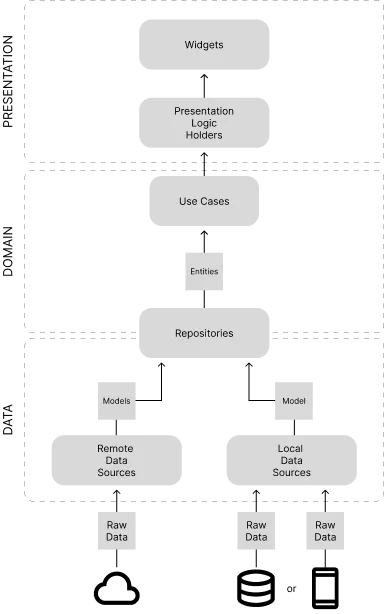
\includegraphics[width=0.5\textwidth]{imagens/cleanarch.png}
        \caption{\scriptsize Exemplificação da arquitetura em camadas}
        \footnotesize  \centering{\textbf{Fonte: Semih Altin\cite{cleanarchitecture}}}
        \label{fig:clean-architecture}
    \end{figure}

    \FloatBarrier

    Embora o Flutter seja capaz de gerar aplicativos nativos para Android e iOS, o aplicativo Encontre na UFMS foi desenvolvido apenas para Android, visto que a Apple, dona do sistema operacional iOS, restringe o desenvolvimento para seu sistema caso o desenvolvedor não possua um dispositivo da marca. Mas, em teoria, o aplicativo poderia ser facilmente adaptado para iOS, bastando apenas compilar o código fonte em um ambiente de desenvolvimento da Apple. O código-fonte do frontend está disponível no repositório em: \textit{Frontend Encontre Na Ufms} \cite{frontend}.

    Uma das grandes preocupações ao se desenvolver um aplicativo móvel é a gerência de possíveis estados enquanto o usuário navega e interage com este aplicativo, como fazer telas conversarem entre si e como manter a experiência o mais contínua e suave possível. Para isso é muito importante separar a apresentação dos dados para o usuário da lógica de negócios que faz todo o tratamento desses dados. A fim de exercer esse papel foi utilizdo o padrão BLoC (Business Logic Component), com a biblioteca \textit{flutter\_bloc} \cite{flutterbloc}, que permite acessar todo o estado da aplicação a qualquer momento e também dispara eventos quando certos estados mudam para que a apresentação dos dados esteja sempre atualizada.

    Para armazenar localmente o token do usuário logado foi utilizado o \textit{Hive} \cite{hive}, um banco de dados não relacional que tem como principais características a leveza e a rapidez. O mini mapa que é utilizado para mostrar a localização e para cadastrar um novo local facilitando o processo para o usuário foi implementado utilizando a biblioteca \textit{google\_maps\_flutter} \cite{googlemapsflutter} desenvolvido pela própria equipe do Flutter. 

\subsubsection{Backend}


    O backend foi desenvolvido utilizando o framework \textit{Fastify} \cite{fastify} com \textit{Node.js} \cite{nodejs}, proporcionando alto desempenho e grande velocidade nas requisições em comparação a outros frameworks, além da facilidade de uso. Foi utilizado \textit{TypeScript} \cite{typescript} para aumentar a segurança contra erros de tipagem durante o processo de desenvolvimento.
    
    Durante o desenvolvimento, foi utilizado a linguagem de programação Typescript para tipagem de variáveis, classes e objetos, evitando eventuais erros que poderiam ser causados por incompatibilidade de tipos. Para a execução do código utilizando o Node.js, foi utilizado uma ferramenta do TypeScript: "tsc" ou TypeScript Compiler, para transpilação do código-fonte em JavaScript durante o desenvolvimento, enquanto que para ser utilizado em produção, foi utilizado o tsup, uma ferramenta de empacotamento e transpilação de código TypeScript para JavaScript, rápida e eficiente.

    O código foi desenvolvido utilizando o padrão de software \textit{MVC ou Model-View-Controller} \cite{mvc}, sendo em português: Modelo-Visão-Controlador. As três camadas se entrelaçam entre si, onde o Controlador recebe as requisições do usuário e as envia para o Modelo, que manipula os dados e faz a conexão com o banco de dados, após, é retornado para o Controlador que envia para a Visão, que exibe as informações ao usuário. Para a comunicação entre o backend e o frontend, foi utilizado uma API REST. O código-fonte do backend está disponível no repositório em: \textit{Backend Encontre Na Ufms} \cite{backend}

\subsubsection{Banco de dados}
    
    Foi utilizado o MySQL, um Sistema de Gerenciamento de Banco de Dados Relacional baseado em SQL, para armazenar e gerenciar os dados do sistema.  Na imagem abaixo, está descrita a estrutura do banco de dados do aplicativo Encontre na UFMS.
    %tambem prefiro o segundo, apagando o texto lá embaixo
    Para o armazenamento de dados no backend, foi utilizado o \textit{MySQL} \cite{mysql}, um sistema de gerenciamento de banco de dados relacional open-source que oferece confiabilidade e desempenho. A conexão entre o Node.js e o MySQL foi feita utilizando o \textit{Drizzle} \cite{drizzle}, um mapeador de objetos (ORM) que foca na velocidade e eficiência na entrega de dados entre as duas ferramentas.

\begin{figure}[h]
    \centering
    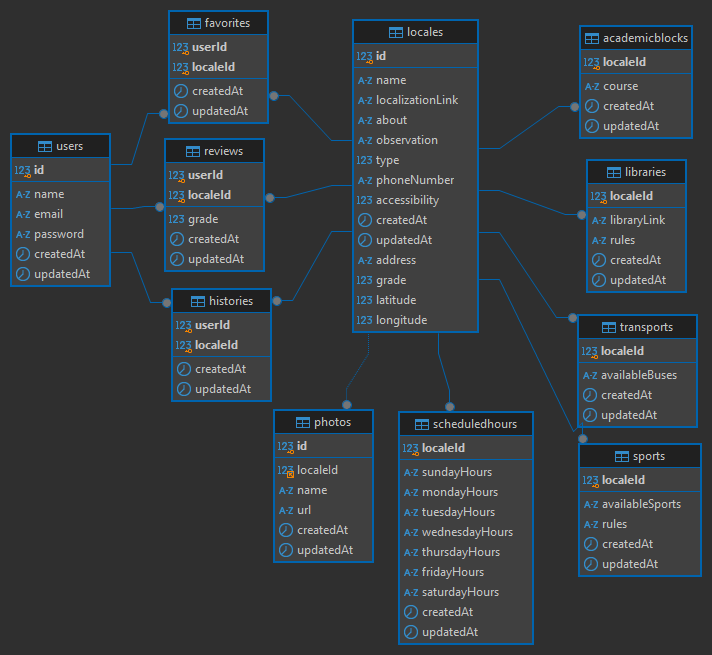
\includegraphics[width=1.1\textwidth]{imagens/encontrenaufms.png}
    \caption{\scriptsize Interface do DBeaver exibindo a estrutura do banco de dados \cite{dbeaver}.}
    \label{fig:descricaoBancoDeDados}
\end{figure}

    Como descrito na Figura 6, o centro da aplicação e do banco de dados são locais. A estrutura do banco foi modelada para permitir uma organização eficiente das informações, com tabelas que representam tanto os locais quanto os atributos e relacionamentos associados:

    \begin{itemize}
        \item \textbf{Locales}: Armazena os dados gerais de cada local, como nome, descrição, e localização.
        \item \textbf{Schedules}: Relacionamento de um para um com a tabela Locales, responsável por armazenar os horários de funcionamento dos locais ao longo da semana.
        \item \textbf{Photos}: Relacionamento de um para muitos com a tabela Locales, onde cada local pode ter diversas fotos associadas.
        \item \textbf{Users}: Armazena os dados do usuário, como nome, email, senha.
        \item \textbf{Histories}: Relacionamento de muitos para muitos com a tabela Locales e a tabela Users, onde cada usuário pode ter um histórico de locais visualizados recentemente.
        \item \textbf{Reviews}: Relacionamento de muitos para muitos com a tabela Locales e a tabela Users, armazena as avaliações de cada usuário feitas aos locais.
        \item \textbf{Favorites}: Relacionamento de muitos para muitos com a tabela Locales e a tabela Users, onde cada usuário pode ter locais favoritos.
        \item \textbf{AcademicBlocks}: Tabela exclusiva para armazenar os nomes dos cursos pertencentes ao respectivo bloco acadêmico.
        \item \textbf{Libraries}: Tabela exclusiva para armazenar as as regras e o link para site externo da biblioteca.
        \item \textbf{Sports}: Tabela exclusiva para armazenar as regras e os esportes disponíveis para serem praticados no centro de esportes.
        \item \textbf{Transportes}: Tabela exlusiva para armazenenar os ônibus que passam no local.
    \end{itemize}

    A tabela ``Locales'' armazena os dados gerais que compõem um determinado local. Sendo que cada local pode possuir horários de funcionamento durante a semana, sendo armazenado na tabela ``Schedules''. Os locais também podem ter fotos, sendo armazenados na tabela ``Photos''.
    
    Os locais foram dividos em tipos específicos para melhor organização dos dados e apresentação ao usuário final, sendo eles: Blocos Acadêmicos, Pontos Turísticos, Bancos, Restaurantes, Serviços de Saúde, Bibliotecas, Centros de Esportes, Transportes, Estacionamentos e Prédios Gerais. Alguns desses tipos posssuem tabelas próprias com informações específicas, como é o caso dos tipos: Blocos Acadêmicos, Bibliotecas, Centros de Esportes e Transportes. 
    
    Além disso, também foi criado uma tabela ``Users'' para armazenar os dados básicos do usuário para cadastro e login do mesmo dentro do sistema. Os usuários possuem 3 relações com a tabela ``Locales'', formando 3 tabelas, sendo elas: ``Histories'', ``Reviews'' e ``Favorites'', que armazenam respectivamente:
    
    \begin{itemize}
        \item O histórico dos 5 últimos locais visualizados recentemente
        \item As avaliações que o usuário fez aos locais 
        \item Os locais favoritos.
    \end{itemize}

    Para a conexão entre o Node.js e o MySQL, foi utilizado o Drizzle que é uma ferramenta de mapeamento de objetos, cujo o foco é a velocidade de entrega de dados entre as duas ferramentas.

\subsection{Login}
    Os usuários tem a possibilidade de se cadastrarem no aplicativo, sendo o cadastro um requisito não obrigatório. Para usuários logados no sistema, são utilizados tokens \textit{JWT (JSON Web Token)} \cite{jwt} para autenticação, garantindo acesso seguro e eficaz ao sistema.
    
    Para o envio de e-mails de recuperação de senha, foi utilizado o \textit{MailJet} \cite{mailjet}, uma ferramenta que fornece acesso a APIs para envio de e-mails e mensagens de texto (SMS).

\subsection{Ambiente de desenvolvimento: Visual Studio Code}
    O ambiente de desenvolvimento escolhido foi o \textit{Visual Studio Code} \cite{visualstudiocode}, uma das IDEs mas utilizadas no mundo graças ao grande número de ferramentas que podem ser integradas nela para aumentar as funcionalidades de desenvolvimento, teste e depuração.
    
    Foi utilizado também o \textit{Android SDK (Software Development Kit)} \cite{androidsdk}, que é um conjunto de ferramentas que permite o desenvolvimento de aplicativos para a plataforma Android. Ele inclui um depurador, bibliotecas, um emulador de dispositivo baseado em \textit{QEMU} \cite{QEMU}, documentação, amostras de código e tutoriais.
    
\subsection{Bibiliotecas e Dependências}
    Diversas bibliotecas e dependências foram utilizadas no desenvolvimento do aplicativo Encontre na UFMS, dentre elas destacam-se:
    
    \begin{itemize}
      \item \textbf{Fastify}: Framework para desenvolvimento de aplicações web com Node.js \cite{fastify}.
      \item \textbf{TypeScript}: Linguagem de programação que extende JavaScript, adicionando tipagem à linguagem \cite{typescript}.
      \item \textbf{tsup}: Empacotador de arquivos TypeScript e JavaScript, utilizado para otimizar e gerar builds \cite{tsup}.
      \item \textbf{MySQL}: MySQL é um sistema de gerenciamento de banco de dados relacional de código aberto baseado em SQL \cite{mysql}.
      \item \textbf{Drizzle}: Mapeador de objetos para conexão entre Node.js e MySQL \cite{drizzle}.
      \item \textbf{MailJet}: Ferramenta para envio de emails e sms \cite{mailjet}.
      \item \textbf{Flutter}: Framework para desenvolvimento de aplicativos móveis \cite{flutter}.
      \item \textbf{Dart}: Linguagem de programação utilizada no Flutter \cite{dart}.
      \item \textbf{hive}: Banco de dados não relacional utilizado para armazenamento local \cite{hive}.
      \item \textbf{google\_maps\_flutter}: Biblioteca para implementação de mapas no Flutter \cite{googlemapsflutter}.
      \item \textbf{flutter\_bloc}: Biblioteca para gerenciamento de estados no Flutter \cite{flutterbloc}.
      \item \textbf{dio}: Biblioteca para requisições HTTP no Flutter \cite{dio}.
    \end{itemize}
    
    Todas essas bibliotecas e dependências, bem como outras que foram especificadas nos projetos do frontend e do backend, foram fundamentais para o desenvolvimento do aplicativo Encontre na UFMS, permitindo a implementação de funcionalidades essenciais e a integração entre o backend e o frontend.

\subsection{Testes e Execução}

    O aplicativo Encontre na UFMS foi testado apenas por nós em diversos dispositivos Android, sendo alguns deles dispositivos físicos aos quais possuímos e outros emulados, a fim de garantir a compatibilidade e o bom funcionamento em diferentes tamanhos de tela e versões do sistema operacional. Foi utilizado o emulador do Android Studio para testar o aplicativo no Pixel 6a na API 33 do Android mas foi principalmente testado em dispositivos físicos, como o Galaxy S21 fe e Xiaomi Note 8 Pro, pela facilidade de uso e para poder verificar a usabilidade real do aplicativo em todo momento.
    
    Os testes foram feitos utilizando as principais funcionalidades do aplicativo, na sequência dos items descritos na tabela 1, sendo que a maior parte dos testes foram feitos realizando repetidas ações que de carregamento de informações, que resultam em novas chamadas de API para o backend, garantindo a consistência do backend em receber a requisição e tratá-la corretamente para retornar os dados ao frontend, além de garantir a consistência do frontend em fazer as requisições para a API corretamente e ao apresentar os dados recebidos ao usuário de forma visual.

\subsubsection{Diagrama de Navegação}

    A Figura 7 ilustra o diagrama de navegação do aplicativo Encontre na UFMS:

    \begin{figure}[h]
        \centering
        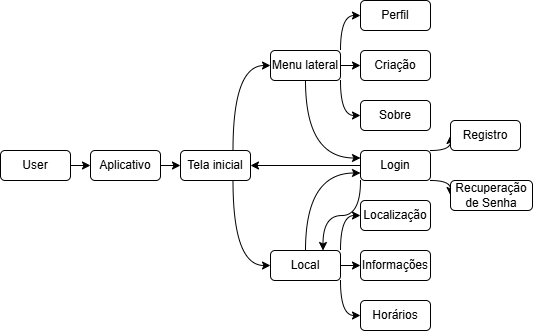
\includegraphics[width=1\textwidth]{imagens/navegacao.png}
        \caption{\scriptsize Diagrama de Navegação}
        \label{fig:diagrama-navegacao}
    \end{figure}

    O diagrama de navegação do aplicativo apresentado acima demonstra os fluxos básicos de navegação que o usuário pode experenciar
    durante o uso do mesmo, vale destacar que algumas telas como Perfil e Criação só são acessíveis caso o usuário esteja logado.

    \FloatBarrier

\subsubsection{Tela 1: Listagem de Locais}

    A tela de listagem de locais é a tela inicial do aplicativo, a primeira e principal tela apresentada para o usuário. Nela, o usuário pode visualizar todos os locais cadastrados no aplicativo, podendo filtrar os locais por categoria e buscar locais através de um campo de pesquisa por texto. 
    
    Cada local é representado por um segmento contendo a foto, o nome, o endereço, a categoria, se o local está provavelmente fechado naquele horário e um indicador que mostra se o local está marcado como favorito ou não. Cada segmento é clicável, redirecionando o usuário para a tela de detalhes do local. O usuário pode também clicar no indicador de favorito para marcar ou desmarcar o local como favorito caso ele esteja logado, caso não esteja o usuário é redirecionando para a tela de Login que será abordada mais a frente. A listagem de locais é paginada, exibindo 10 locais por vez, uma nova requisição é feita toda vez que o usuário chega ao final da lista, carregando a próxima página, se houver.

    Na parte superior da tela há uma seção com um botão, que abre o menu lateral, e um campo de texto para pesquisa. Logo abaixo há um filtro de categorias, uma série de botões que podem ser arrastados horizontalmente, permitindo que o usuário filtre os locais por uma ou mais categorias, de acordo com suas necessidades. Na busca por texto foi aplicado um \textit{debounce} de 1s para evitar que a busca seja feita a cada caractere digitado, o que poderia causar um consumo excessivo de recursos da API. A Figura 8 mostra a tela de listagem de locais.

    \begin{figure}[h]
        \centering
        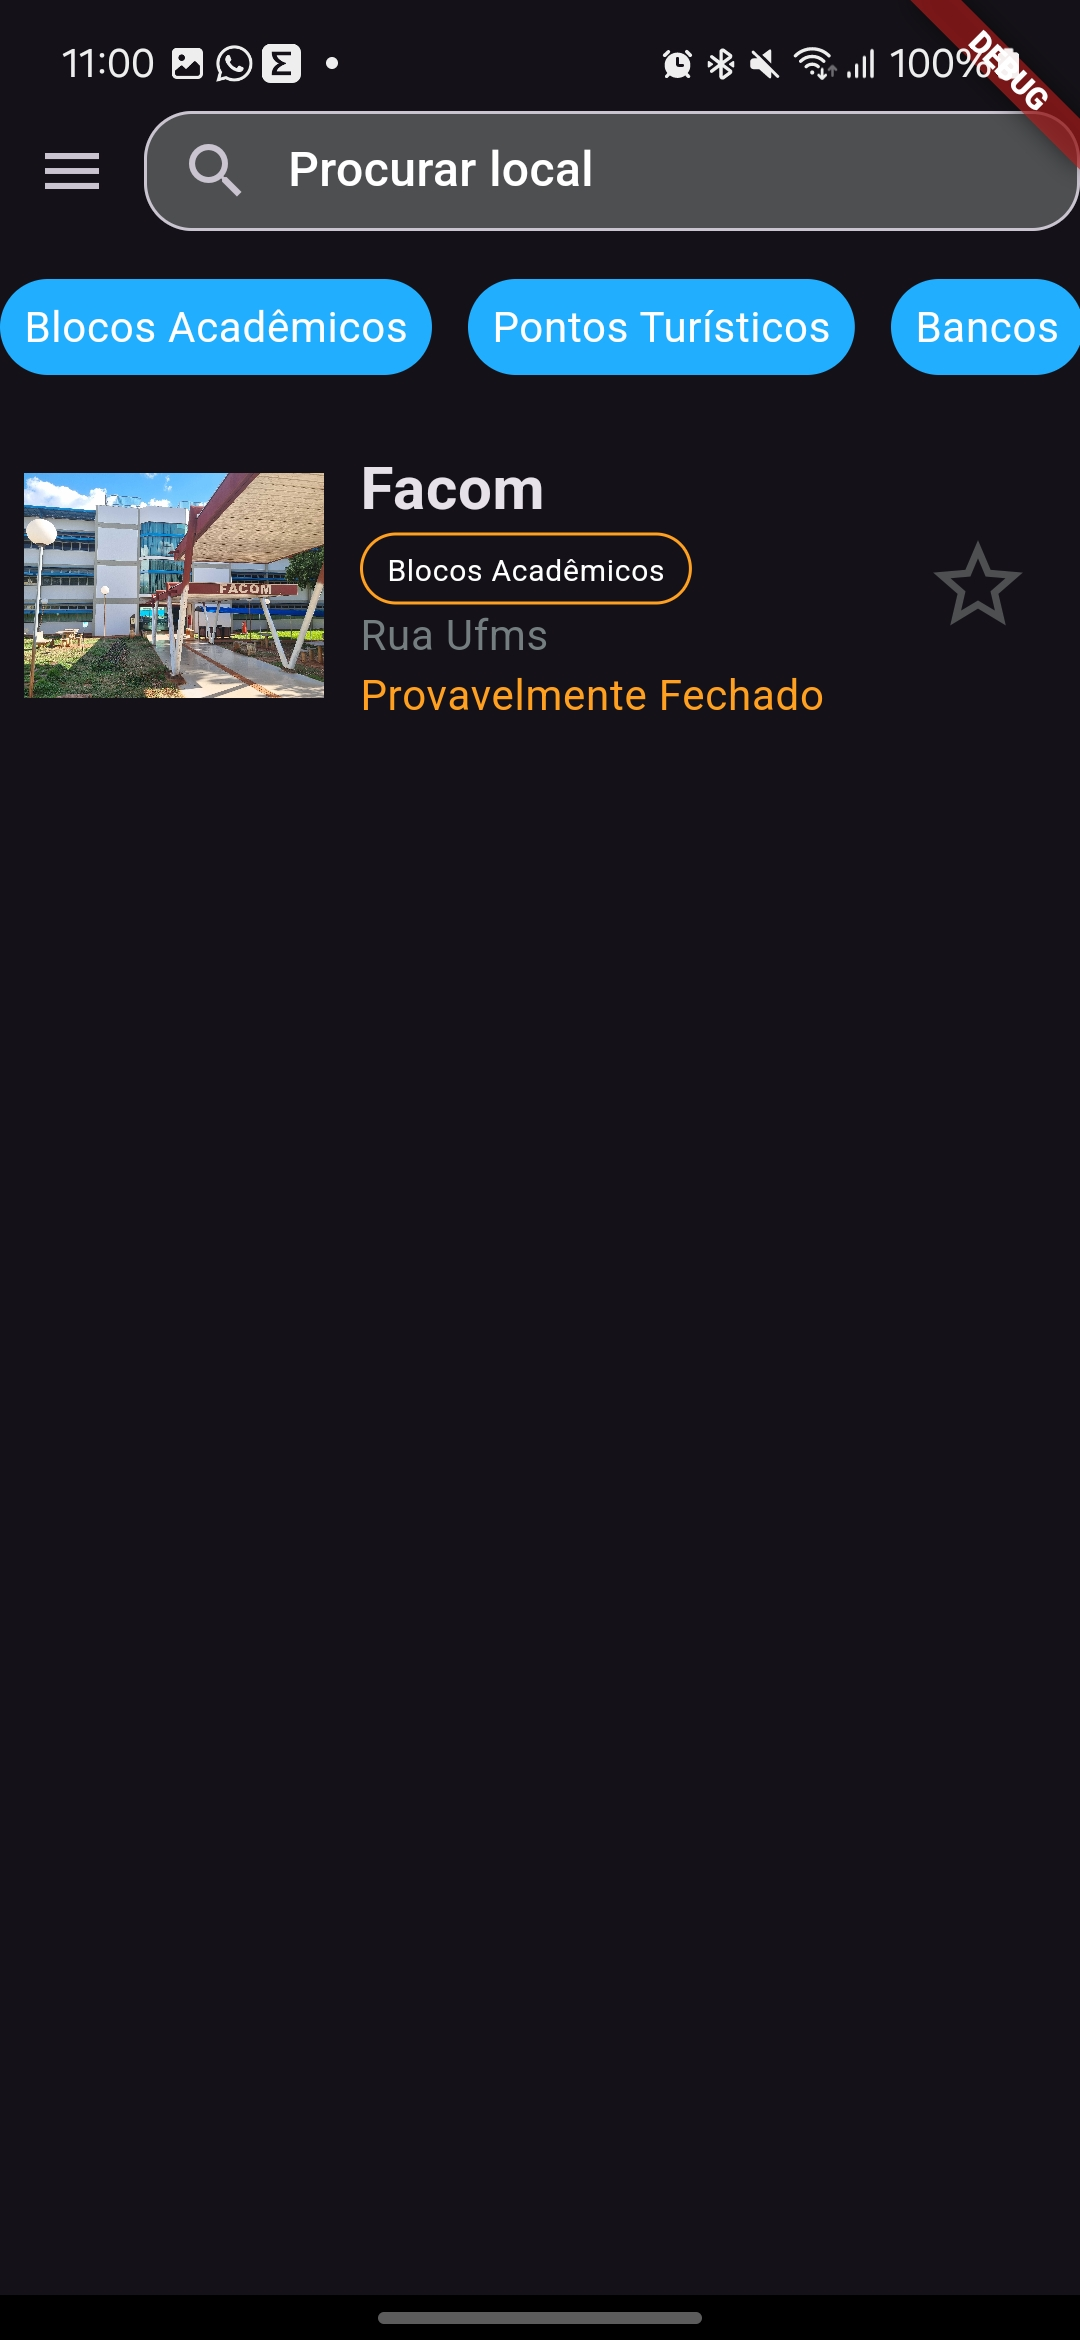
\includegraphics[width=0.4\textwidth]{imagens/inicial.jpg}
        \caption{\scriptsize Tela 1: Listagem de Locais}
        \label{fig:tela1}
    \end{figure}

    \FloatBarrier

\subsubsection{Tela 2: Local}

    A tela de local apresenta todos os detalhes do local que foi selecionado pelo usuário. Nela, o usuário pode visualizar uma ou mais fotos do local, o nome, um indicador que é mostrado caso o local tenha opções de acessibilidade e a avaliação média do local, que é a média das avaliações por outros usuários. Além disso existem 3 abas que o usuário pode navegar sem sair da tela. A aba de localização é a aba inicial e mostra o endereço do local, um mapa com a localização do local indicada e uma seção para o usuário dar sua própria avaliação do local, caso esteja logado. A aba de informações exibe alguns detalhes do local como observações e telefone de contato. Por fim, a aba de Horários exibe os horários de funcionamento do local, caso estejam cadastrados. A Figura 9 mostra a tela de local com a aba de localização, já a Figura 10 apresenta as demais abas.

    \begin{figure}[h]
        \centering
        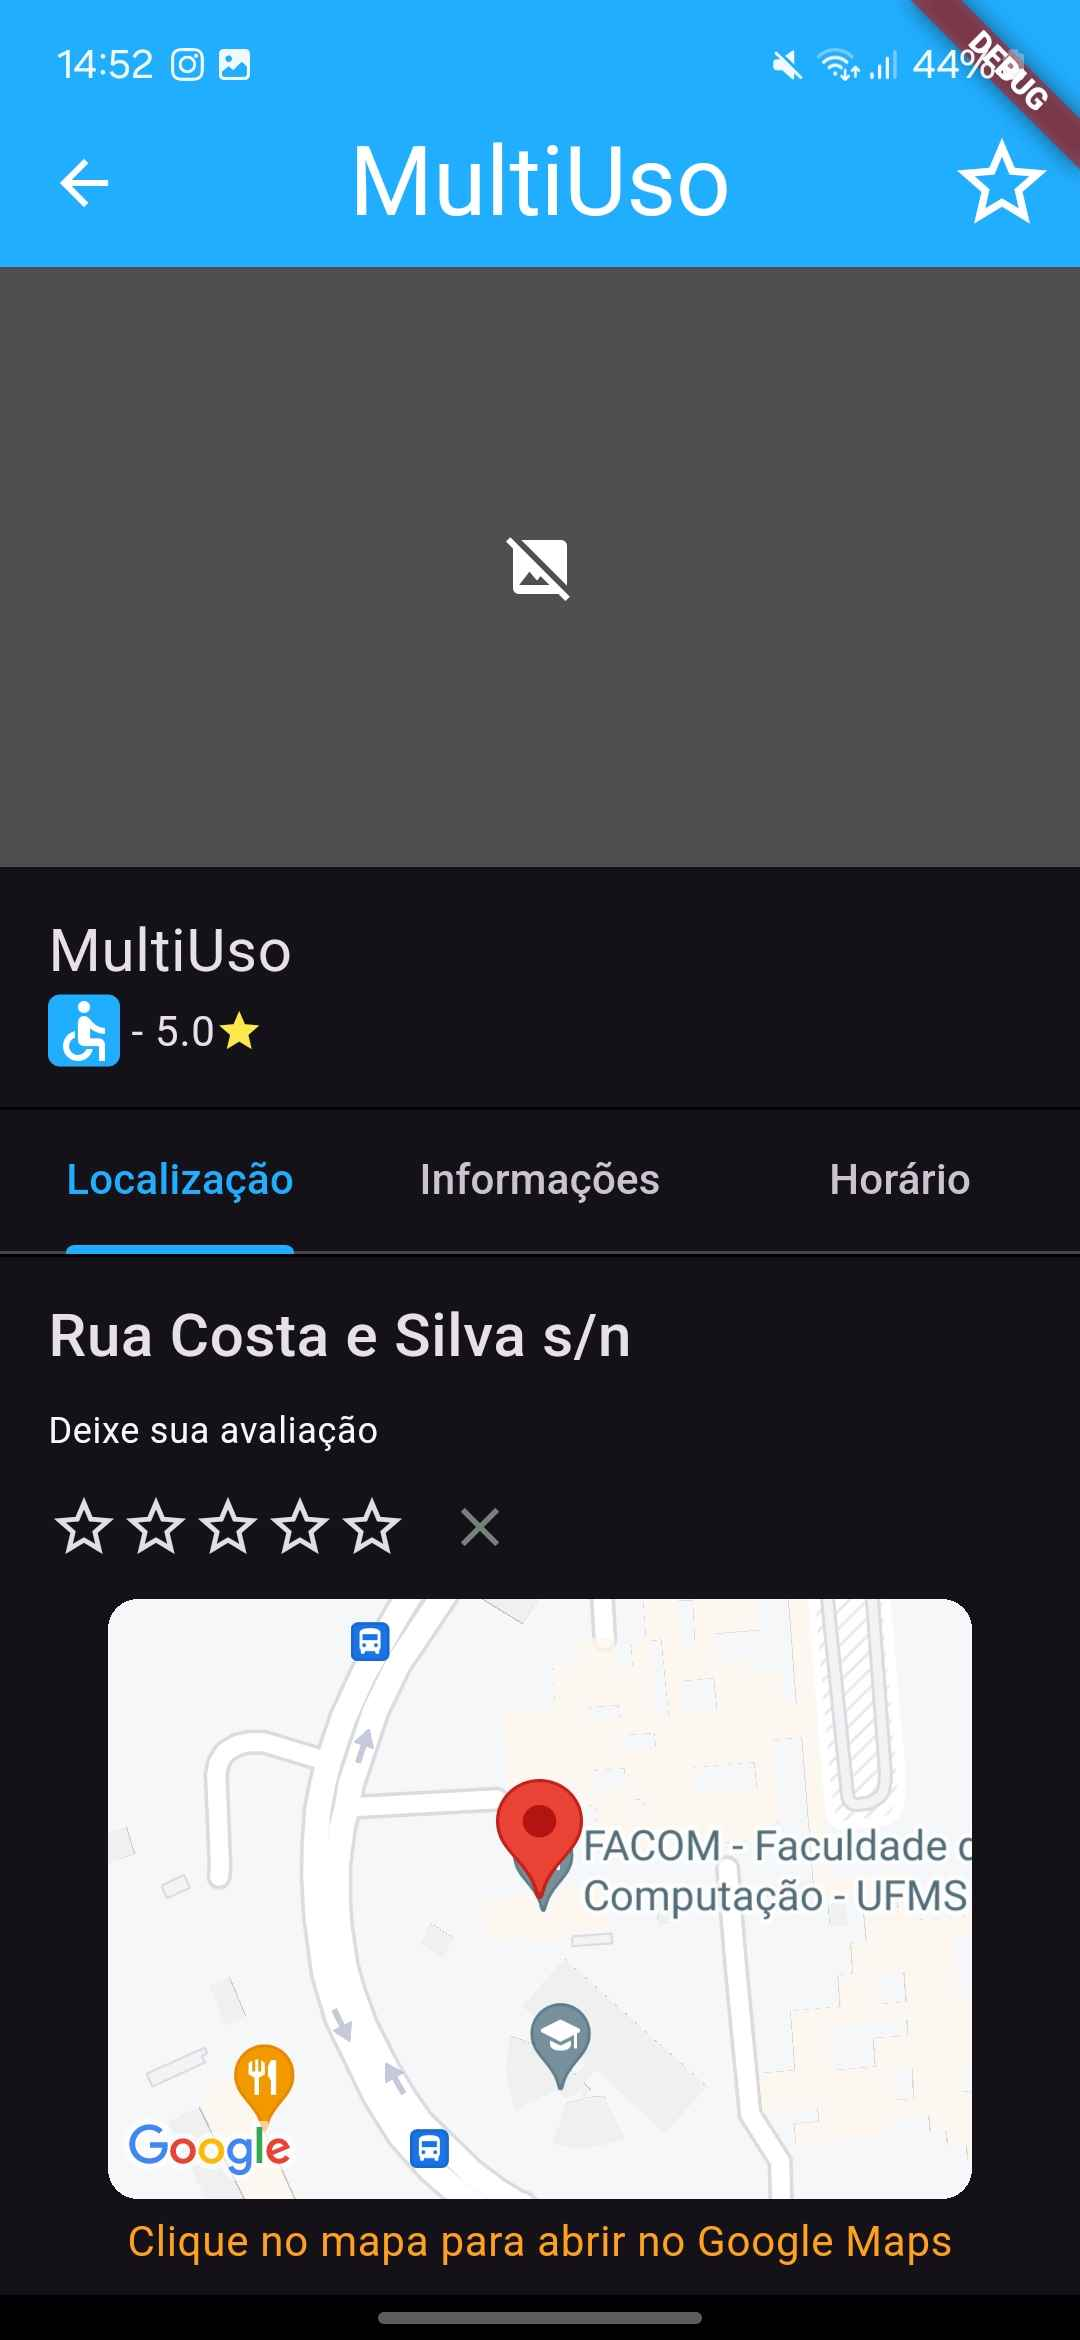
\includegraphics[width=0.4\textwidth]{imagens/local.jpg}
        \caption{\scriptsize Tela 2: Local}
        \label{fig:tela2}
    \end{figure}

    \begin{figure}
        \centering
        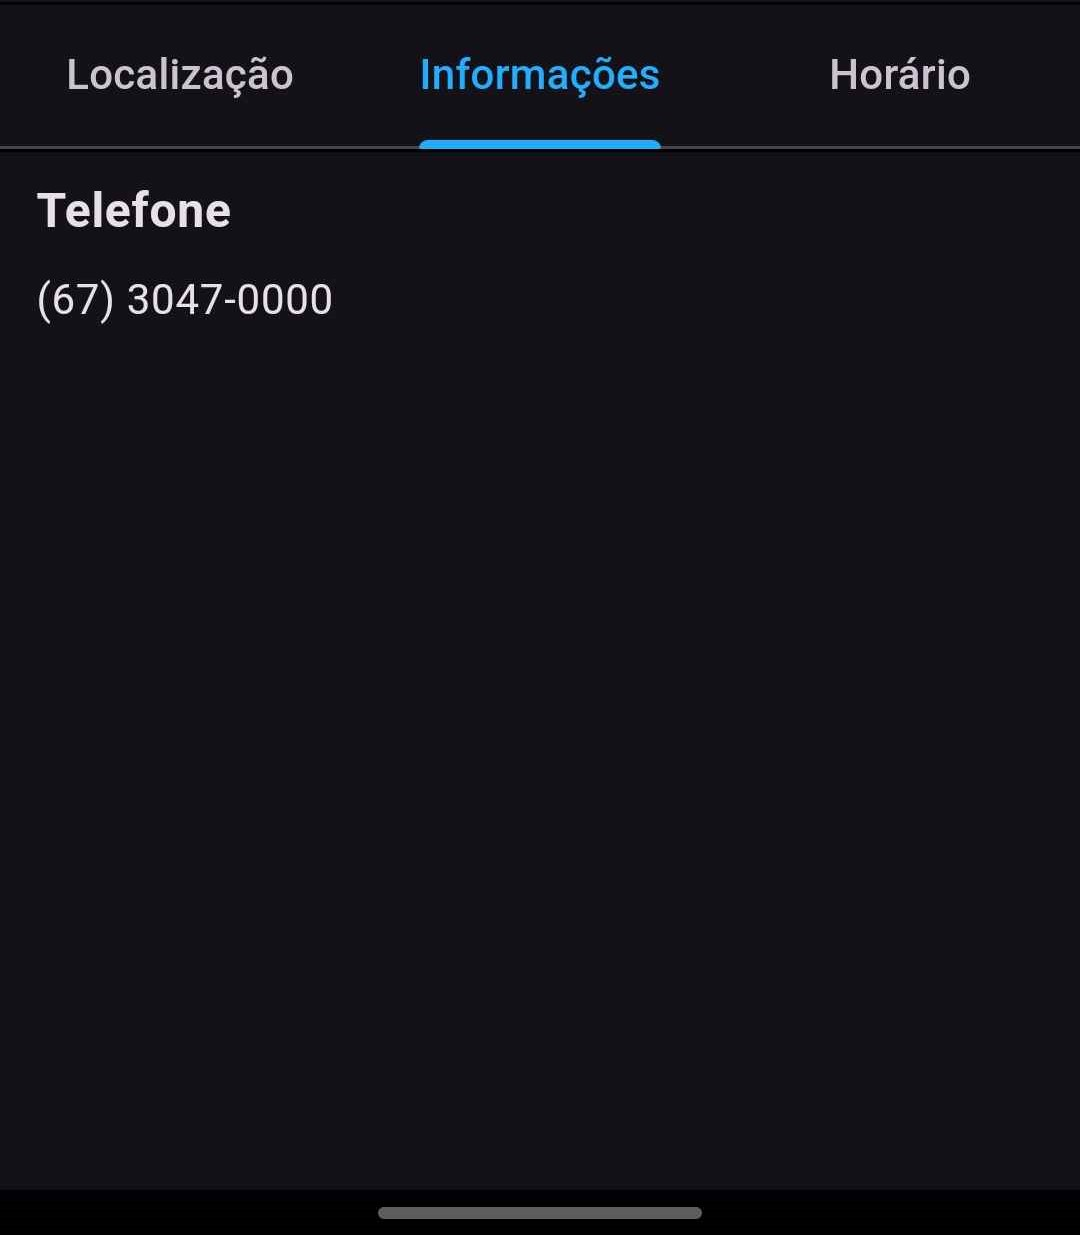
\includegraphics[width=0.4\textwidth]{imagens/info.jpg}
        \hspace{10mm}
        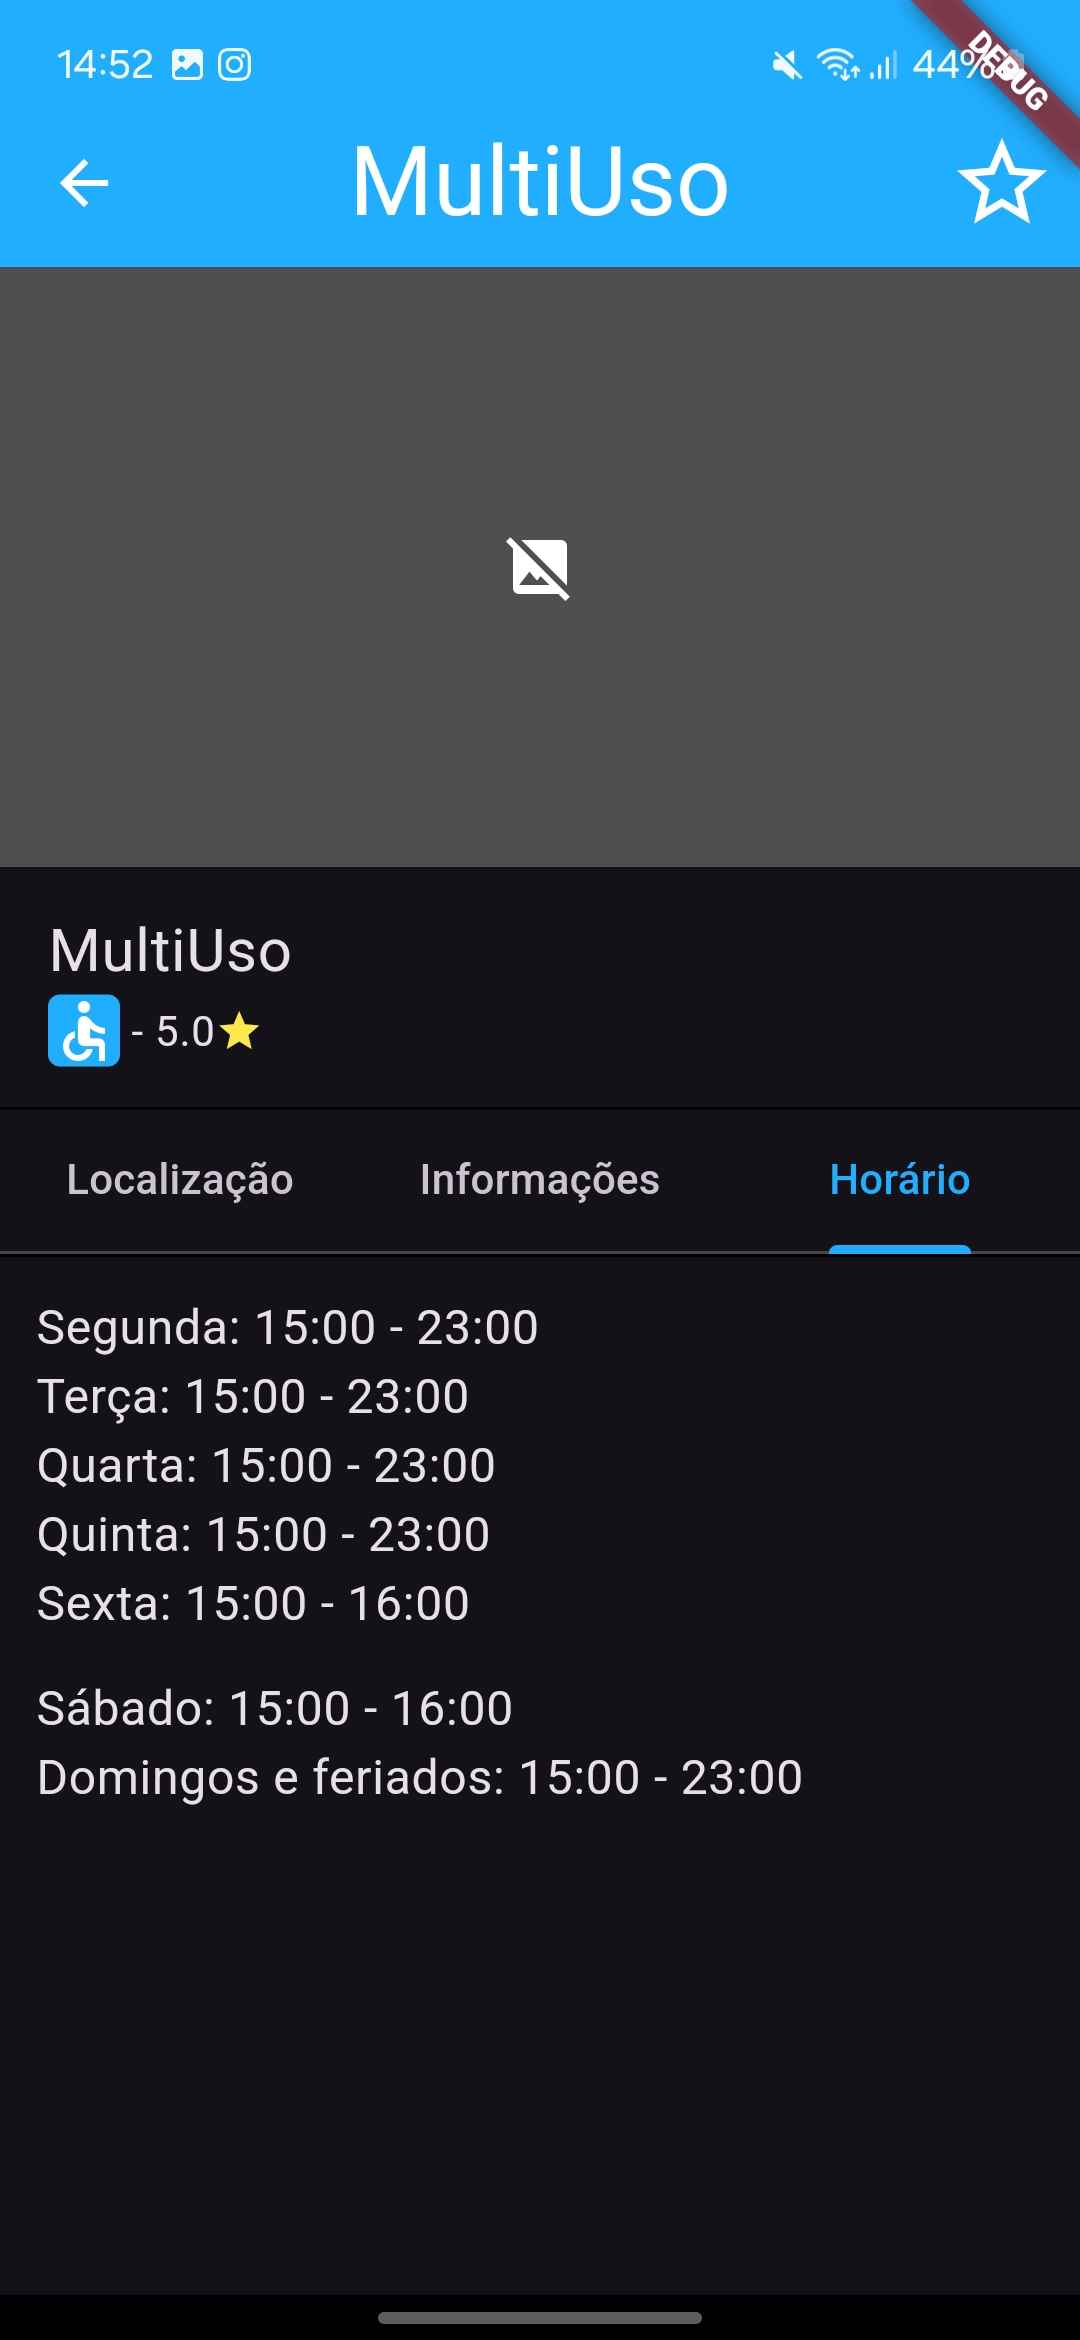
\includegraphics[width=0.4\textwidth]{imagens/horario.jpg}
        \caption{\scriptsize Abas: Informações e Horários}
        \label{fig:tela2-abas}
    \end{figure}

    \FloatBarrier

\subsubsection{Tela 3: Menu Lateral}

    O menu lateral é acessível através de um botão na parte superior da tela de listagem de locais. Ele é composto por uma série de botões que redirecionam o usuário para diferentes telas do aplicativo. O menu lateral é uma forma de organizar as funcionalidades do aplicativo de forma intuitiva e acessível, permitindo que o usuário navegue facilmente entre as diferentes telas do aplicativo.

    Essa tela muda de acordo com o estado de autenticação do usuário, caso ele esteja logado, aparecerá o nome do usuário logo abaixo o nome do aplicativo e os botões de Perfil e Criação assim como um botão de Sair, caso contrário, todas essas informações são omitidas e apenas o botão de Sobre é exibido, e no lugar do botão de Sair é exibido o botão de Login. Abaixo as duas figuras exemplificam ambos os estados. A Figura 11 mostra o menu lateral tanto no estado logado quanto no estado deslogado.

    \begin{figure}[h]
        \centering
        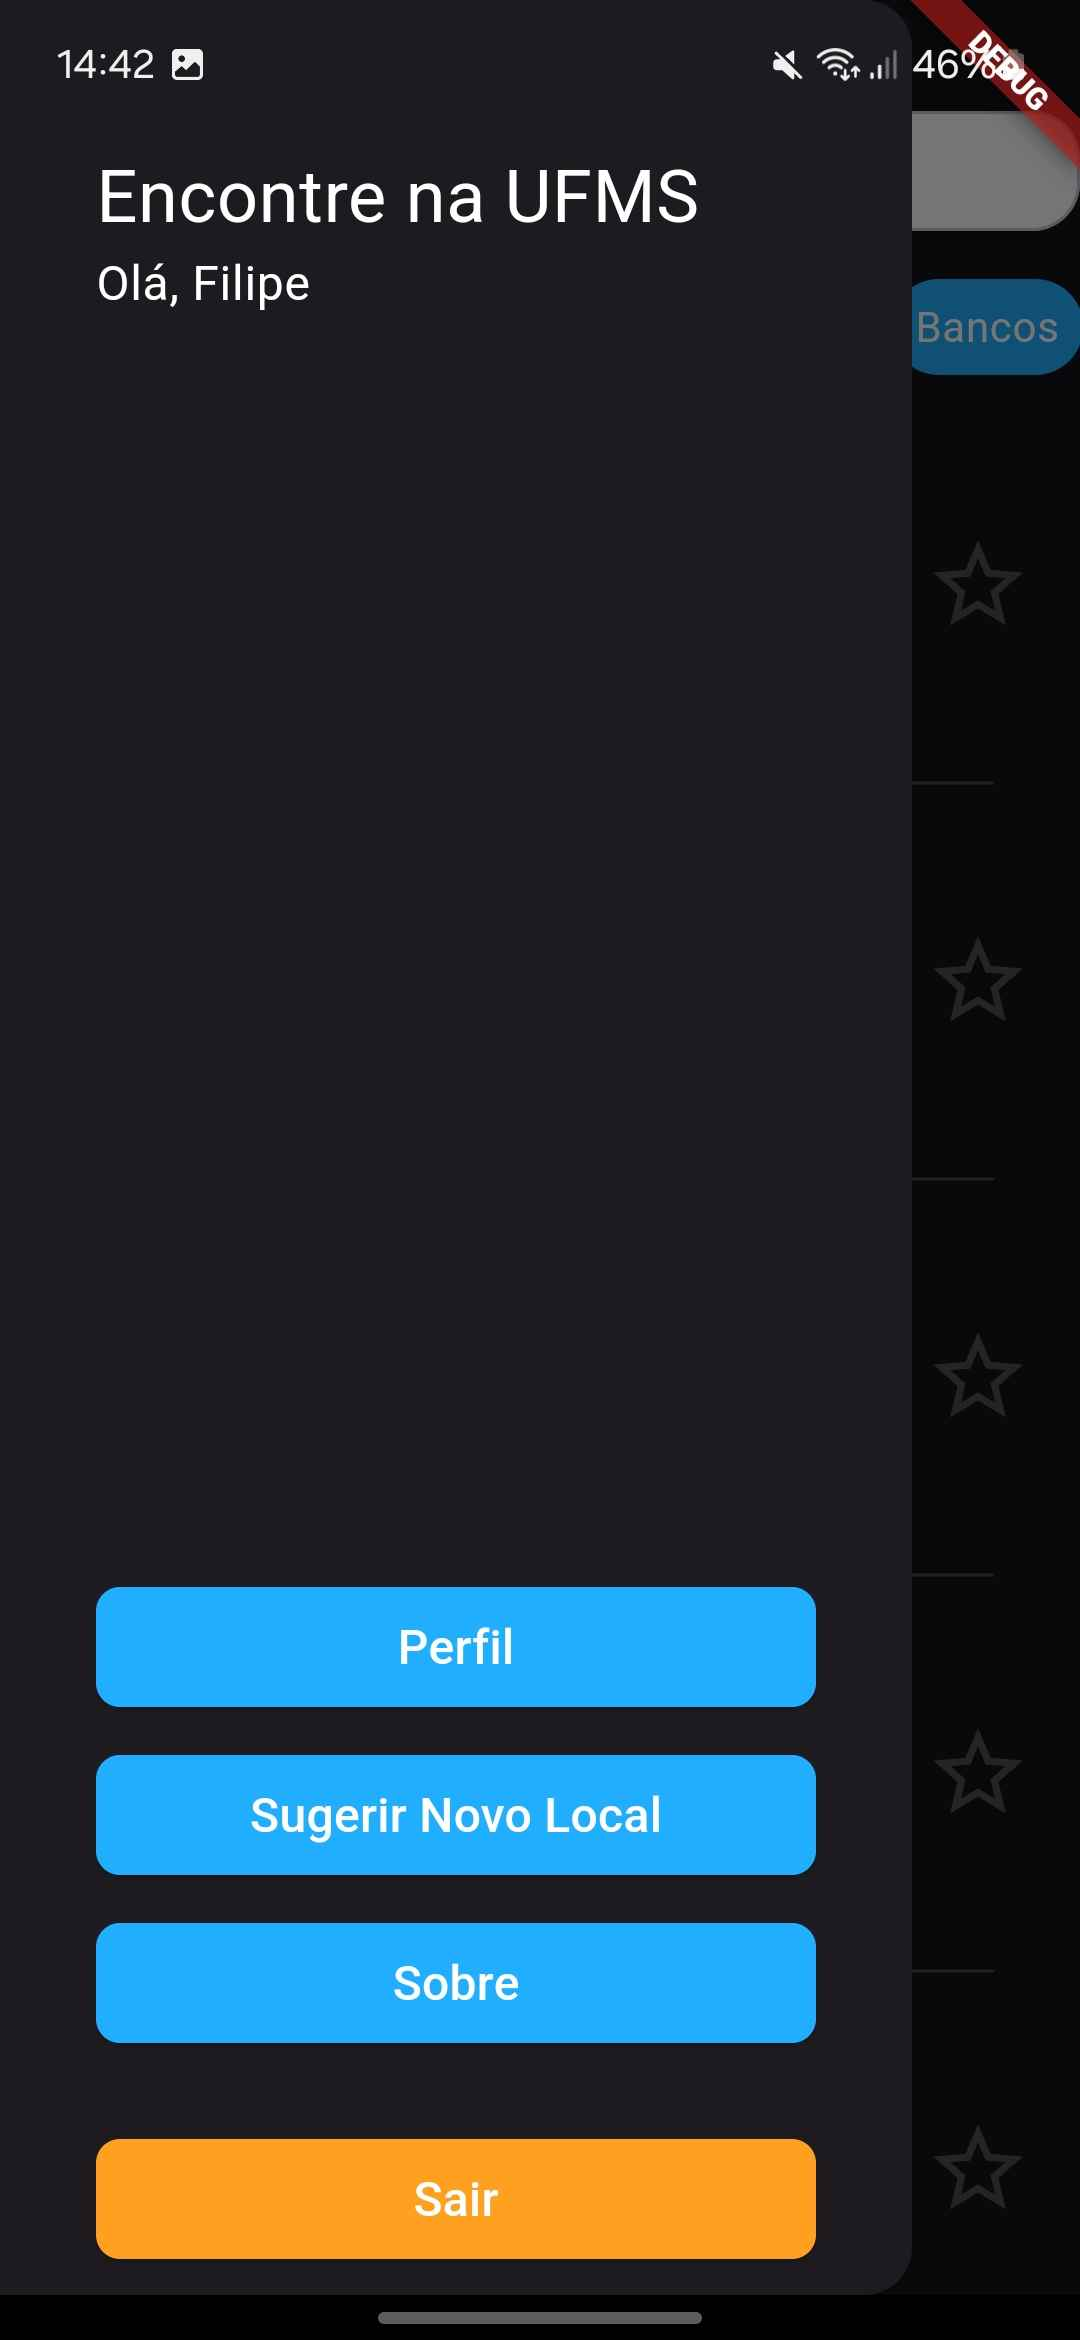
\includegraphics[width=0.4\textwidth]{imagens/menu-lateral-logado.jpg}
        \hspace{10mm}
        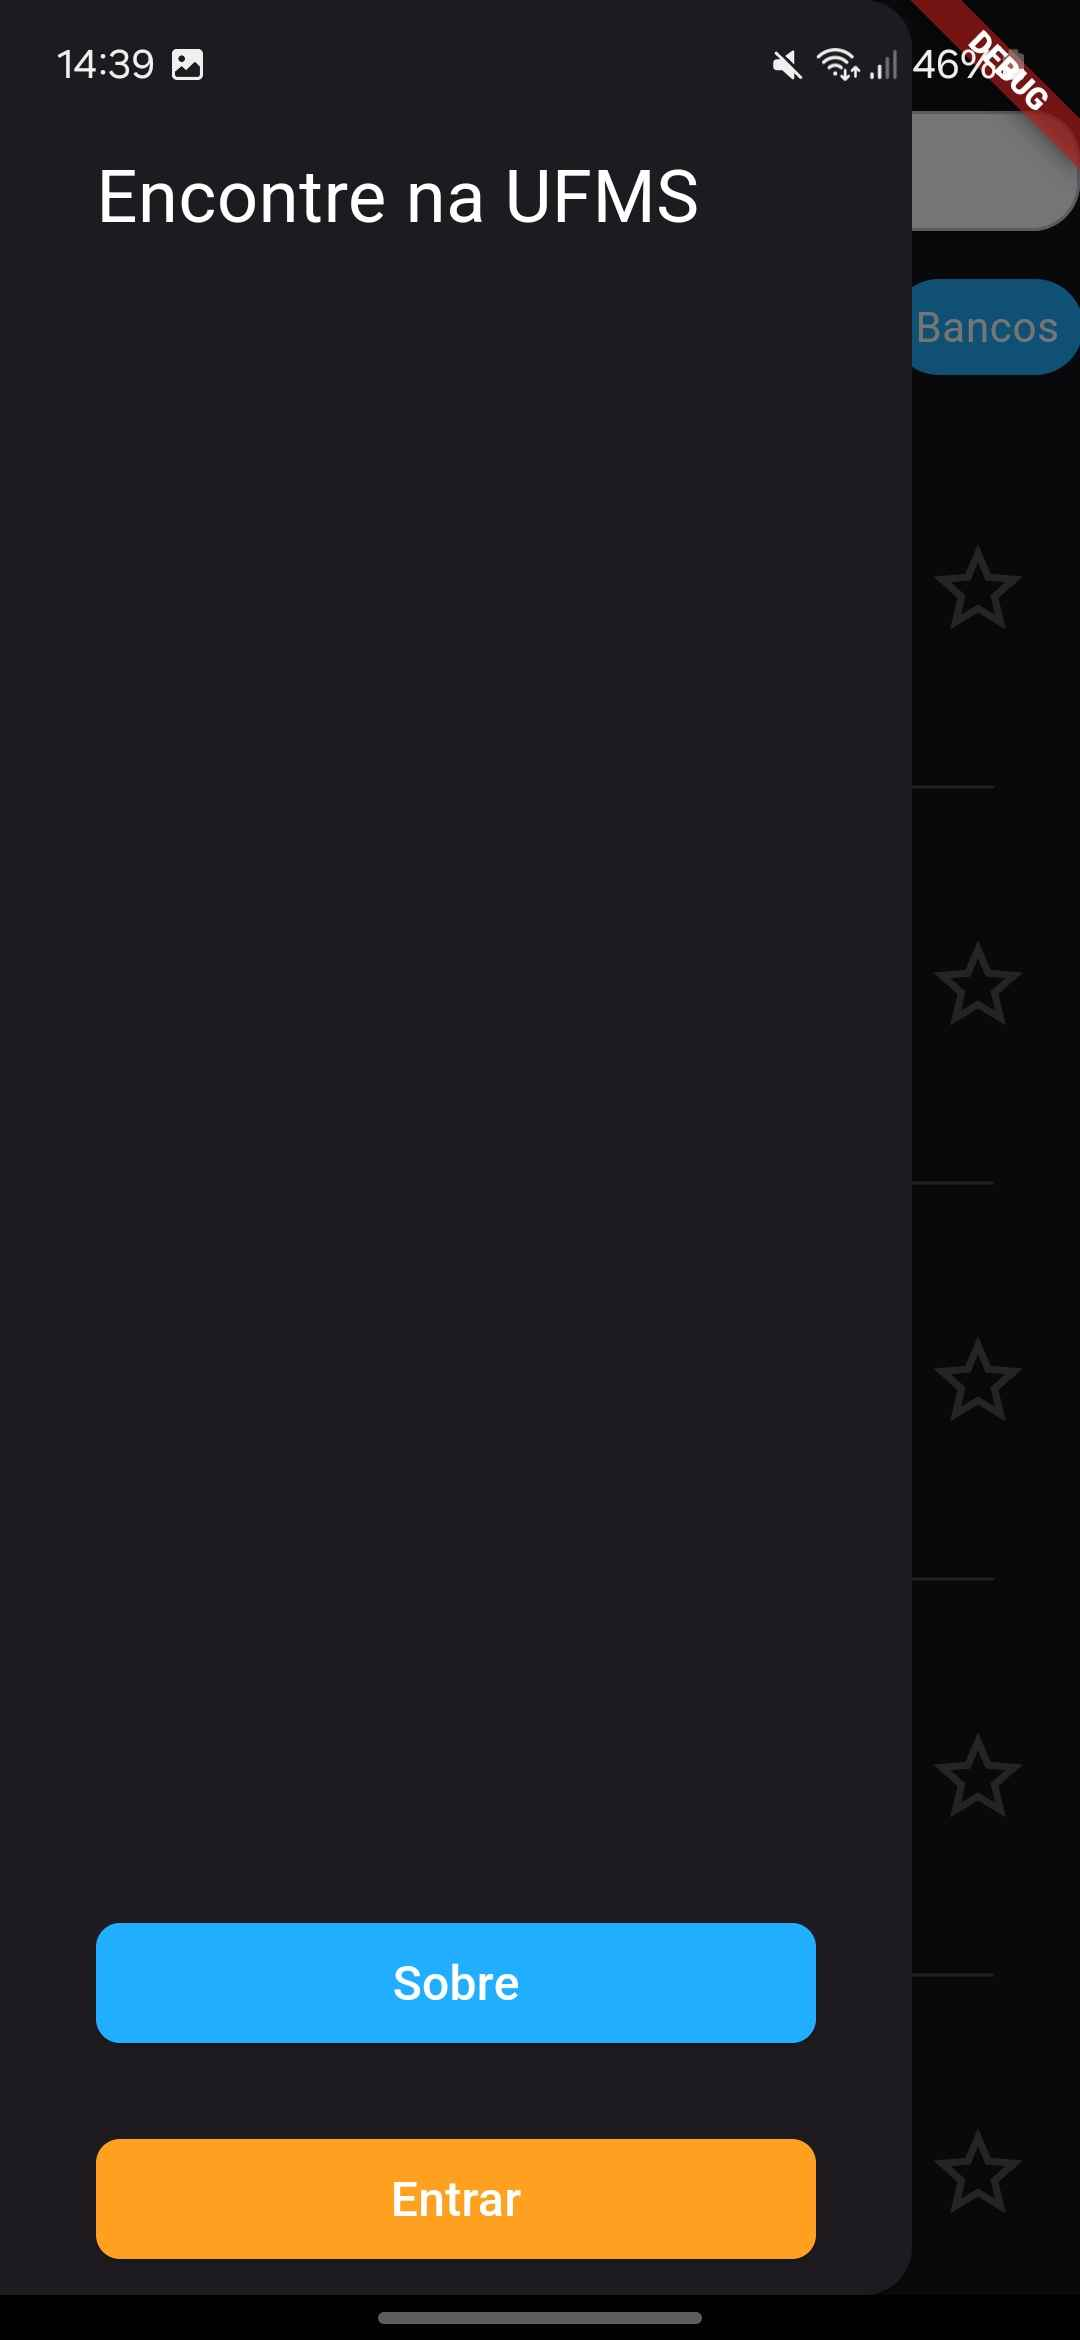
\includegraphics[width=0.4\textwidth]{imagens/menu-lateral-logout.jpg}
        \caption{\scriptsize Tela 2: Menu Lateral (Logado e Deslogado)}
        \label{fig:tela2-logado}
    \end{figure}

    \FloatBarrier

\subsubsection{Tela 4: Perfil}

    A tela de perfil exibe as informações do usuário logado, nome e e-mail. Além disso, a tela também permite que o usuário edite seu nome e altere sua senha. A tela de perfil é uma forma de o usuário gerenciar suas informações pessoais e garantir que seus dados estejam sempre atualizados. A Figura 12 mostra a tela de perfil.

    \begin{figure}[h]
        \centering
        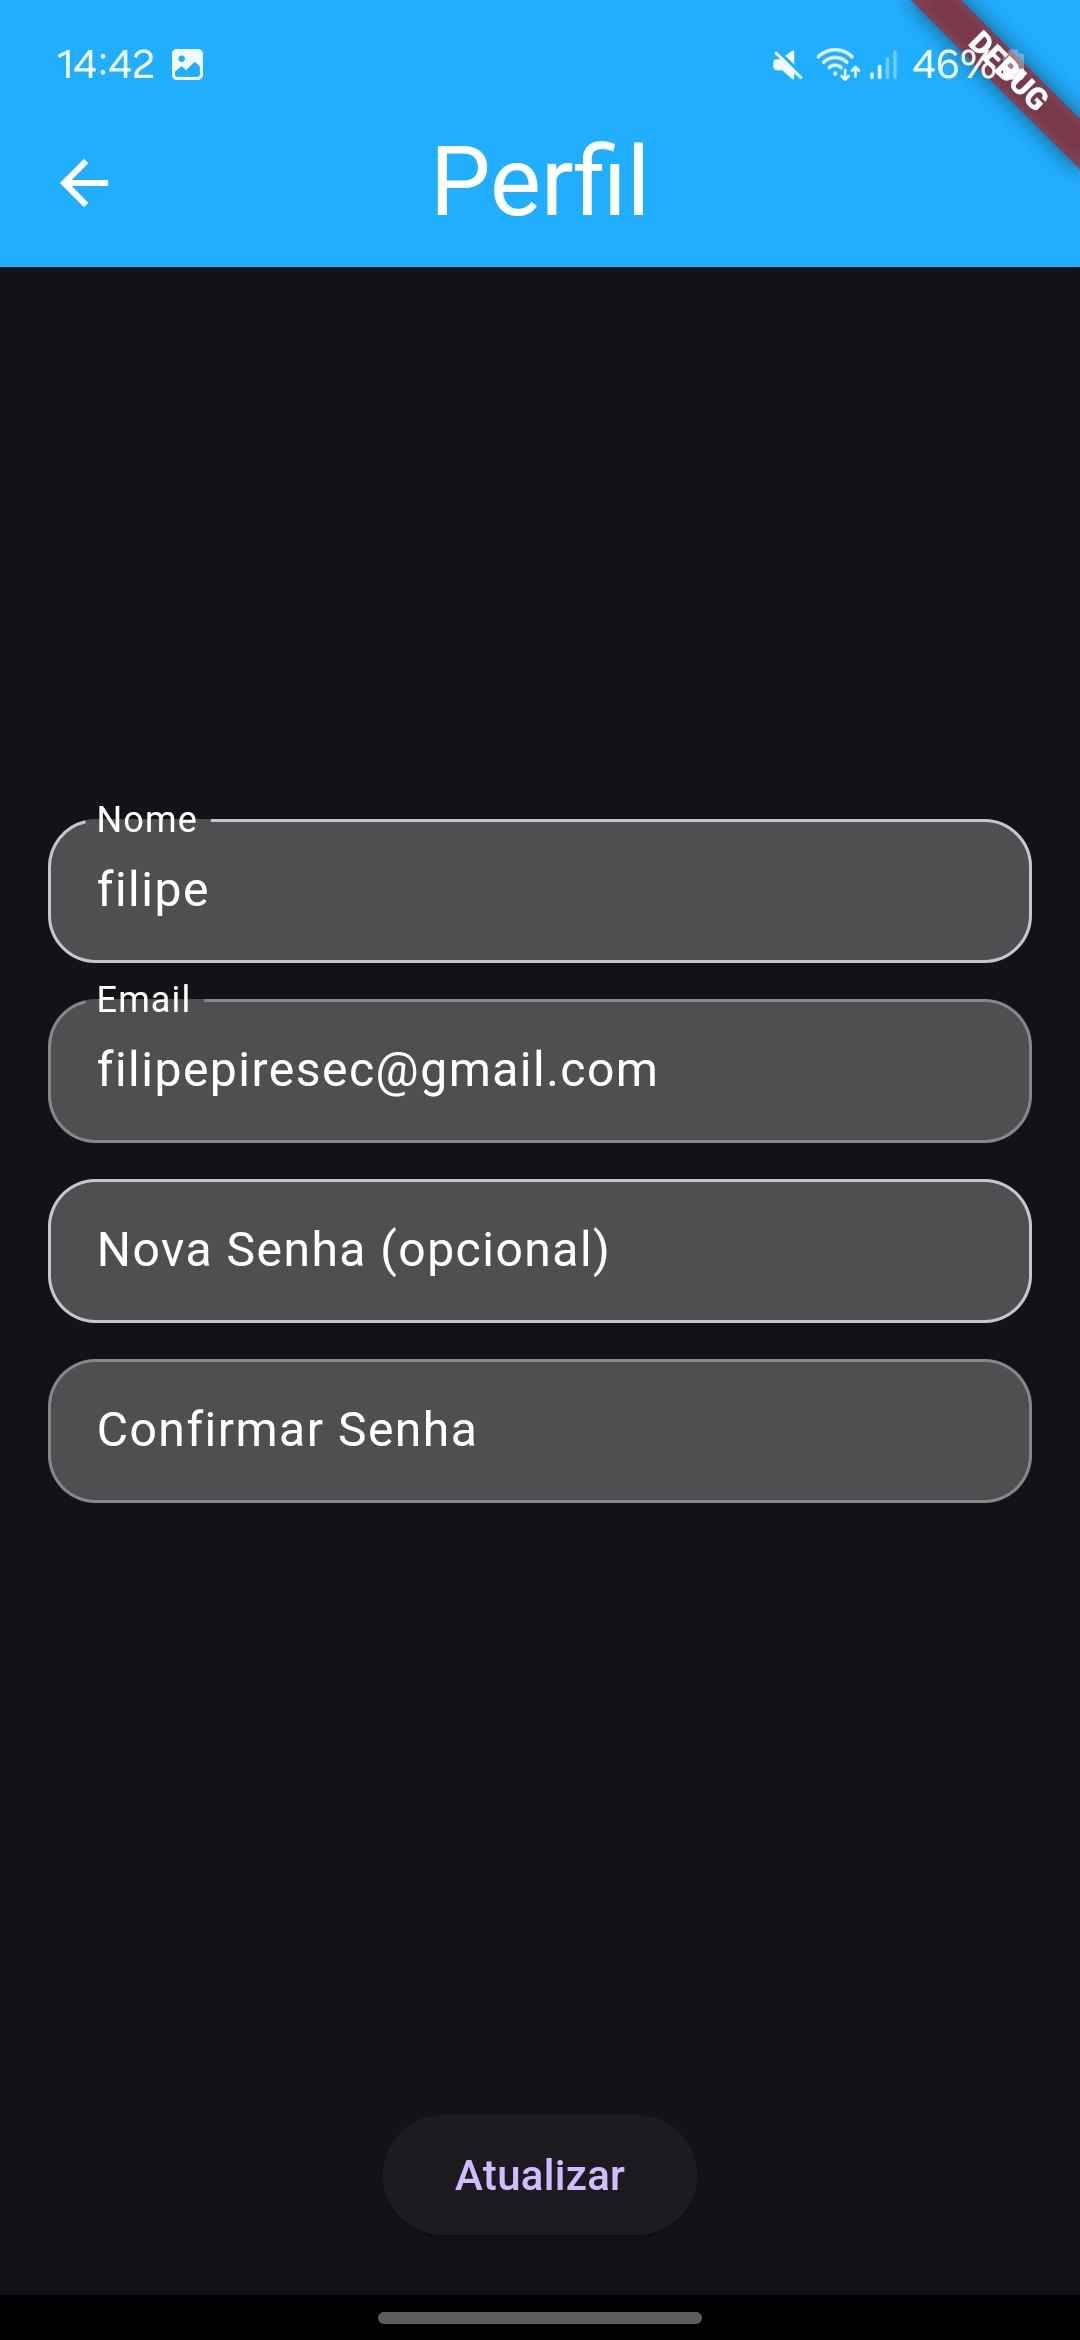
\includegraphics[width=0.4\textwidth]{imagens/perfil.jpg}
        \caption{\scriptsize Tela 4: Perfil}
        \label{fig:tela4}
    \end{figure}

    \FloatBarrier

\subsubsection{Tela 5: Criação}

    A tela de criação possibilita que os usuários preencham uma série de informações sobre o local que desejam cadastrar, como nome, endereço, categoria, horários de funcionamento, telefone de contato, observações e fotos, e enviem para uma avaliação. A tela de criação é uma forma de os usuários contribuírem com o aplicativo, adicionando novos locais e enriquecendo a base de dados do sistema. A Figura 13 mostra as telas de criação.

    \begin{figure}[h]
        \centering
        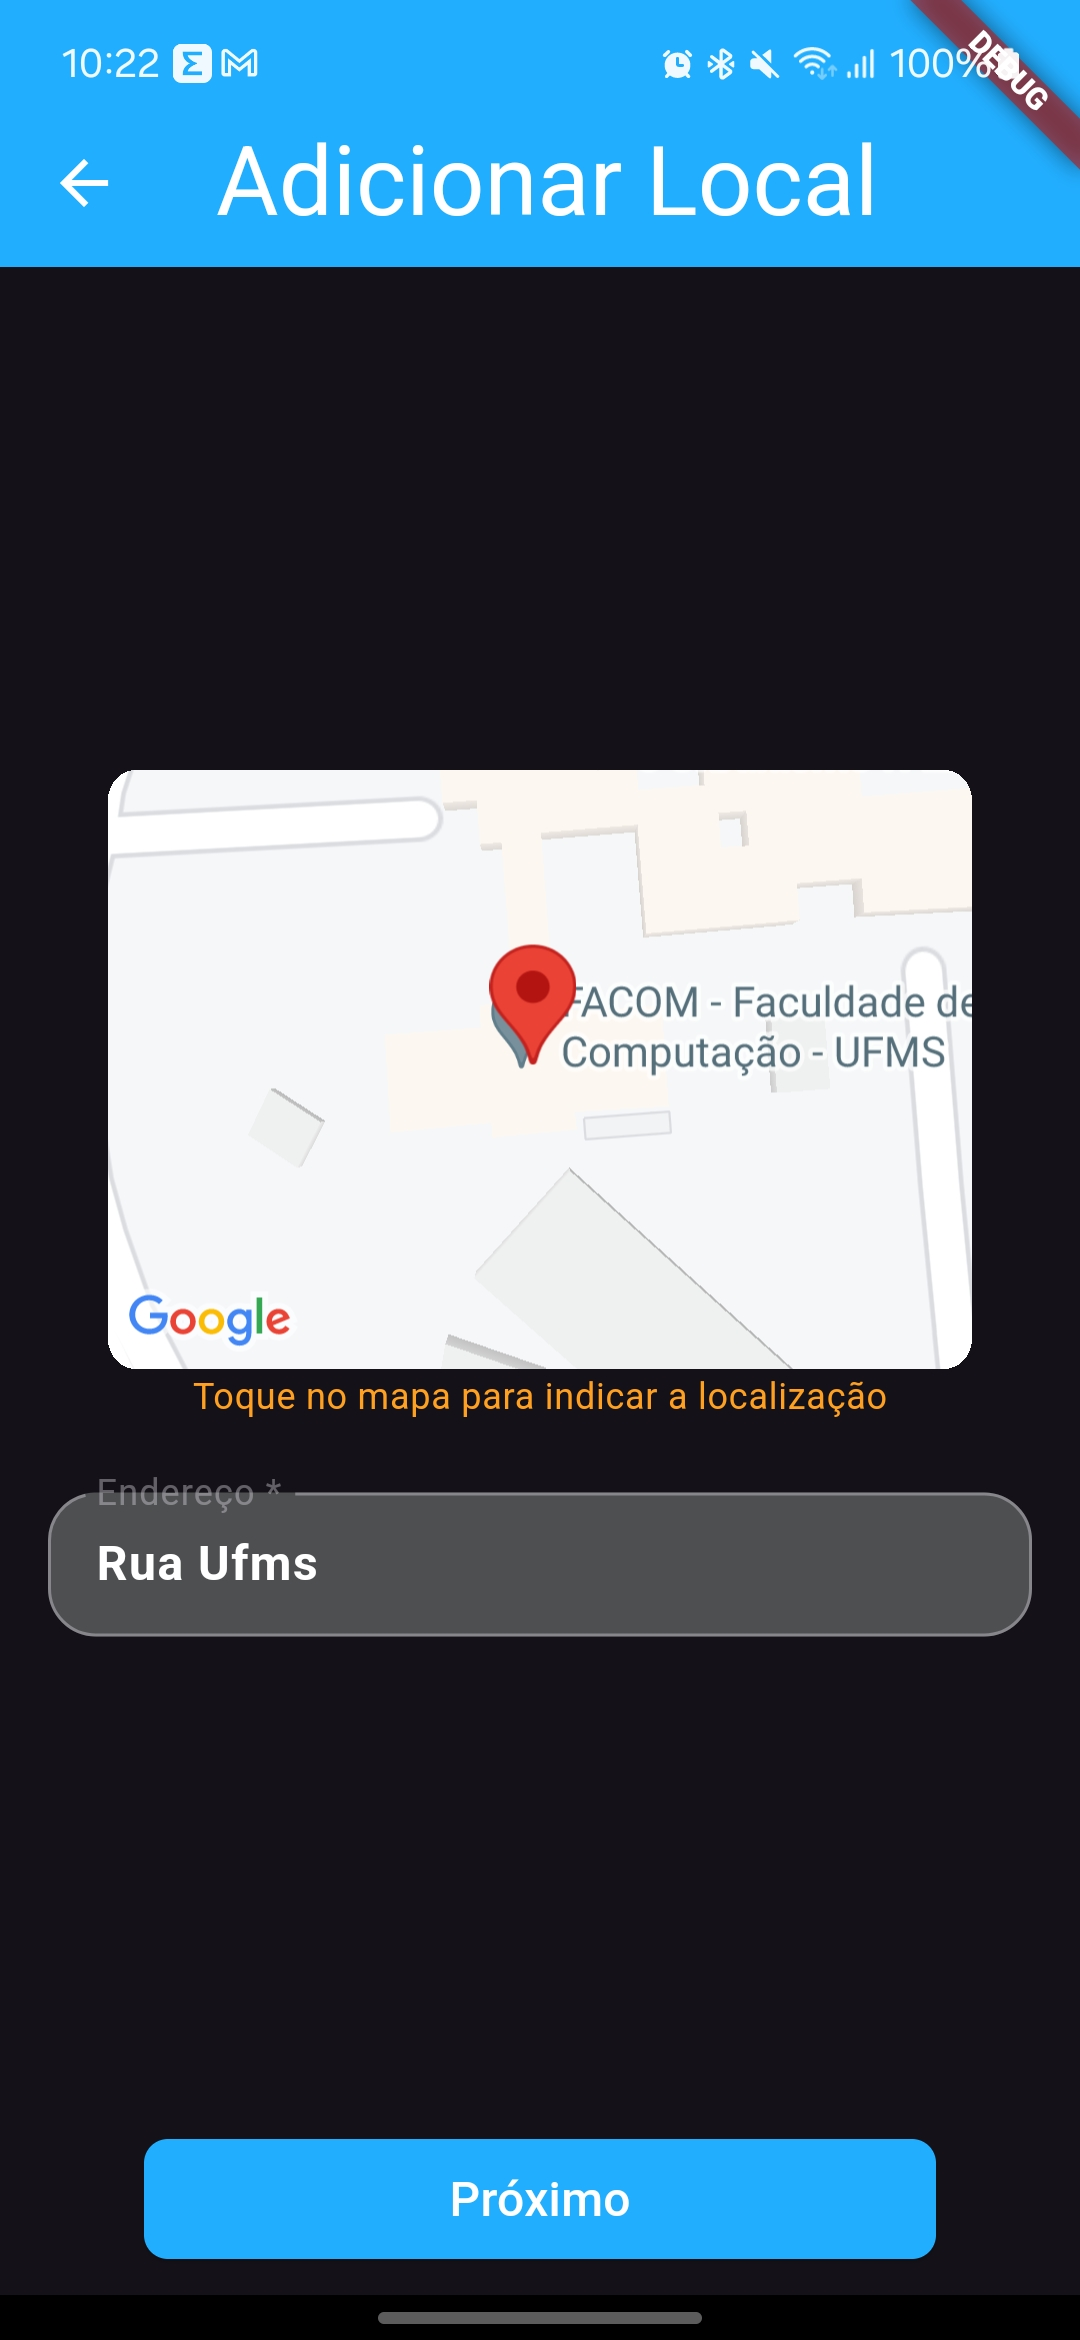
\includegraphics[width=0.4\textwidth]{imagens/criacao.jpg}
        \hspace{10mm}
        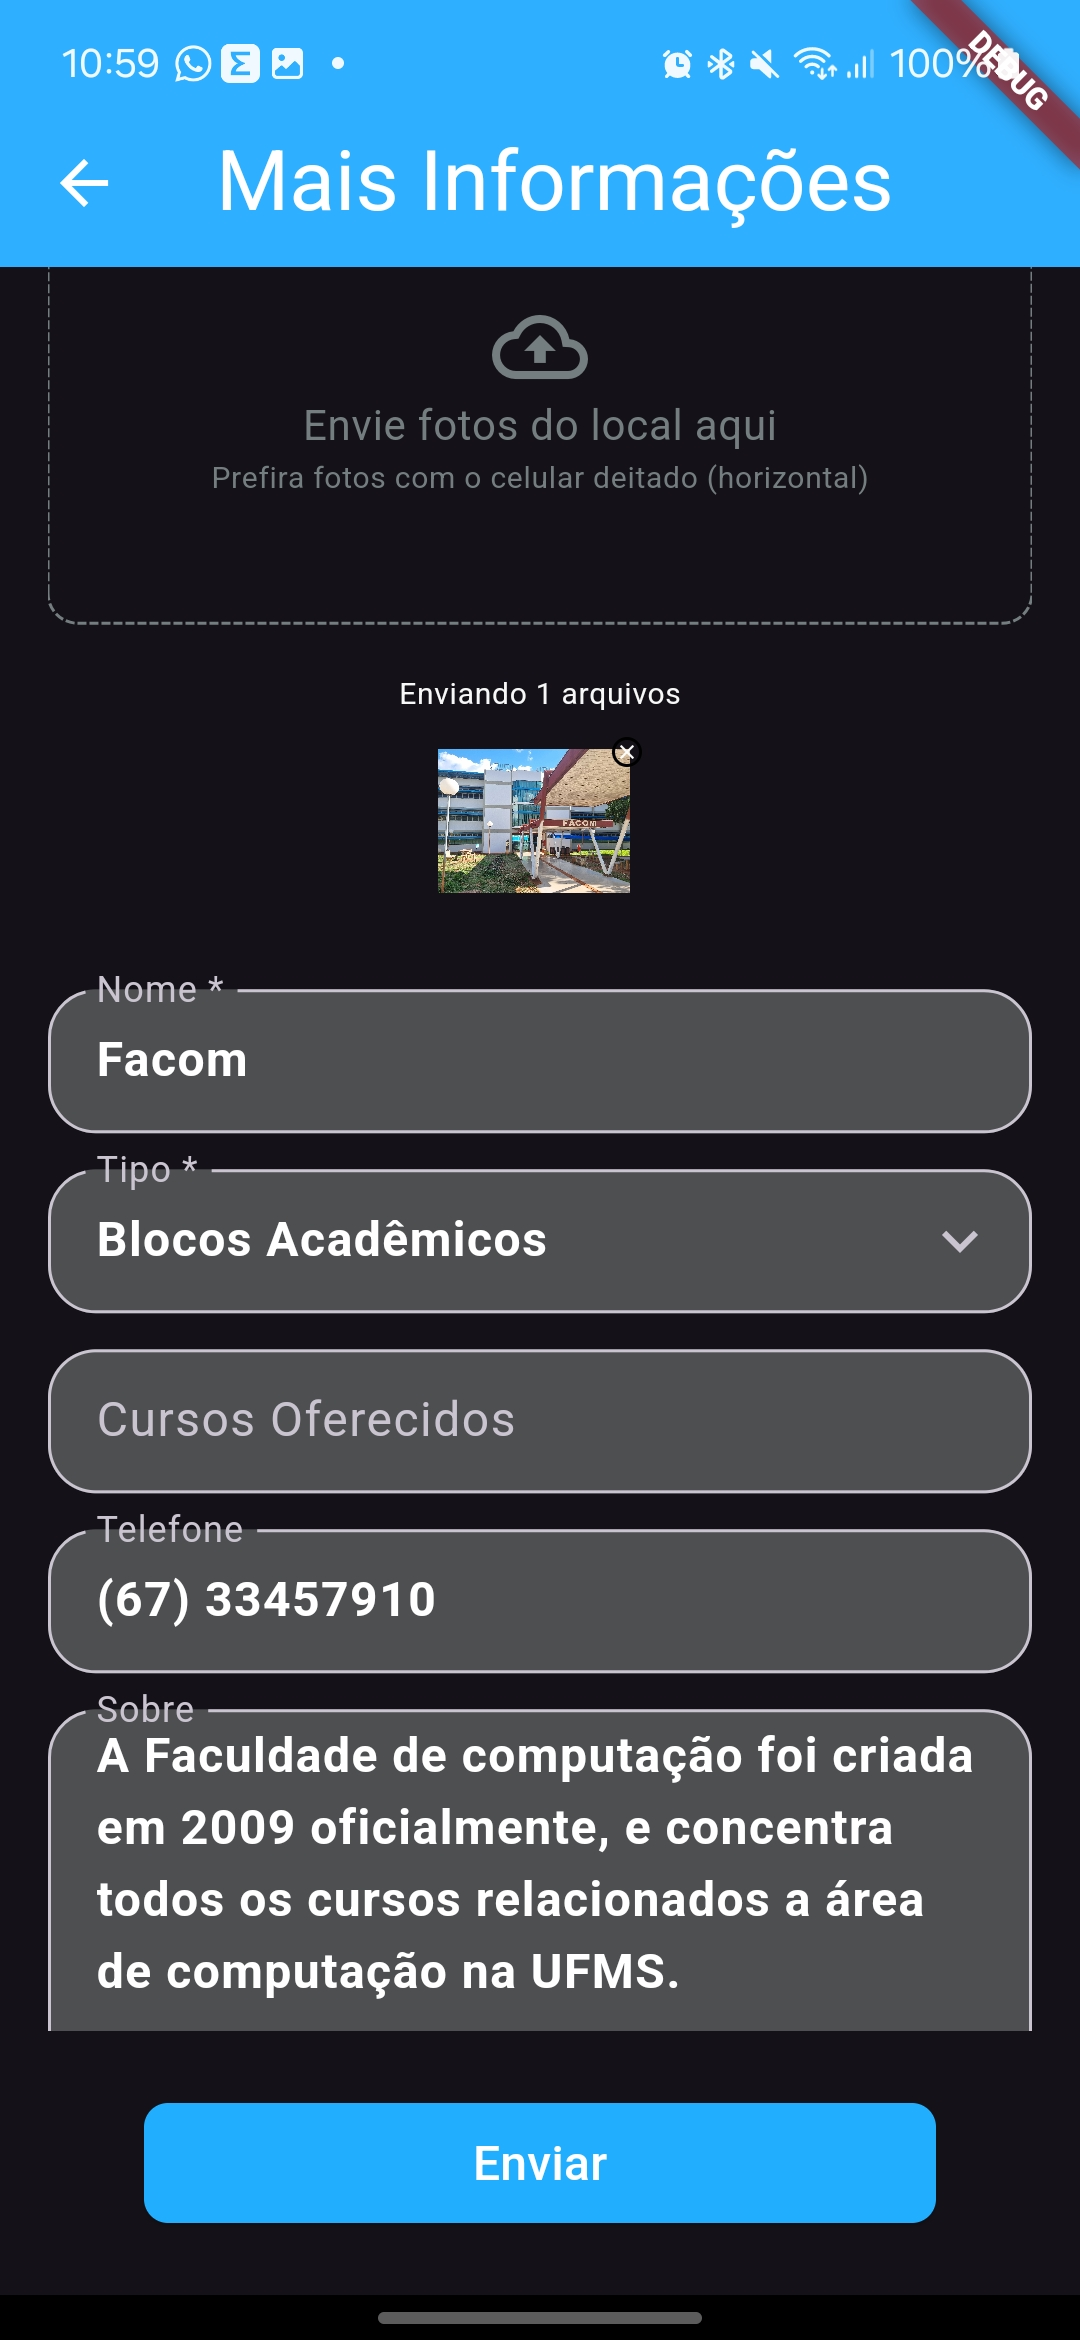
\includegraphics[width=0.4\textwidth]{imagens/criacao2.jpg}
        \caption{\scriptsize Tela 5: Criação}
        \label{fig:tela5}
    \end{figure}

    \FloatBarrier

\subsubsection{Tela 6: Sobre}

    A tela de sobre exibe informações sobre o aplicativo, como a versão, os desenvolvedores e o código fonte. A tela de sobre é uma forma de os usuários conhecerem mais sobre o aplicativo e os desenvolvedores por trás dele. A Figura 14 mostra a tela de sobre.

    \begin{figure}[h]
        \centering
        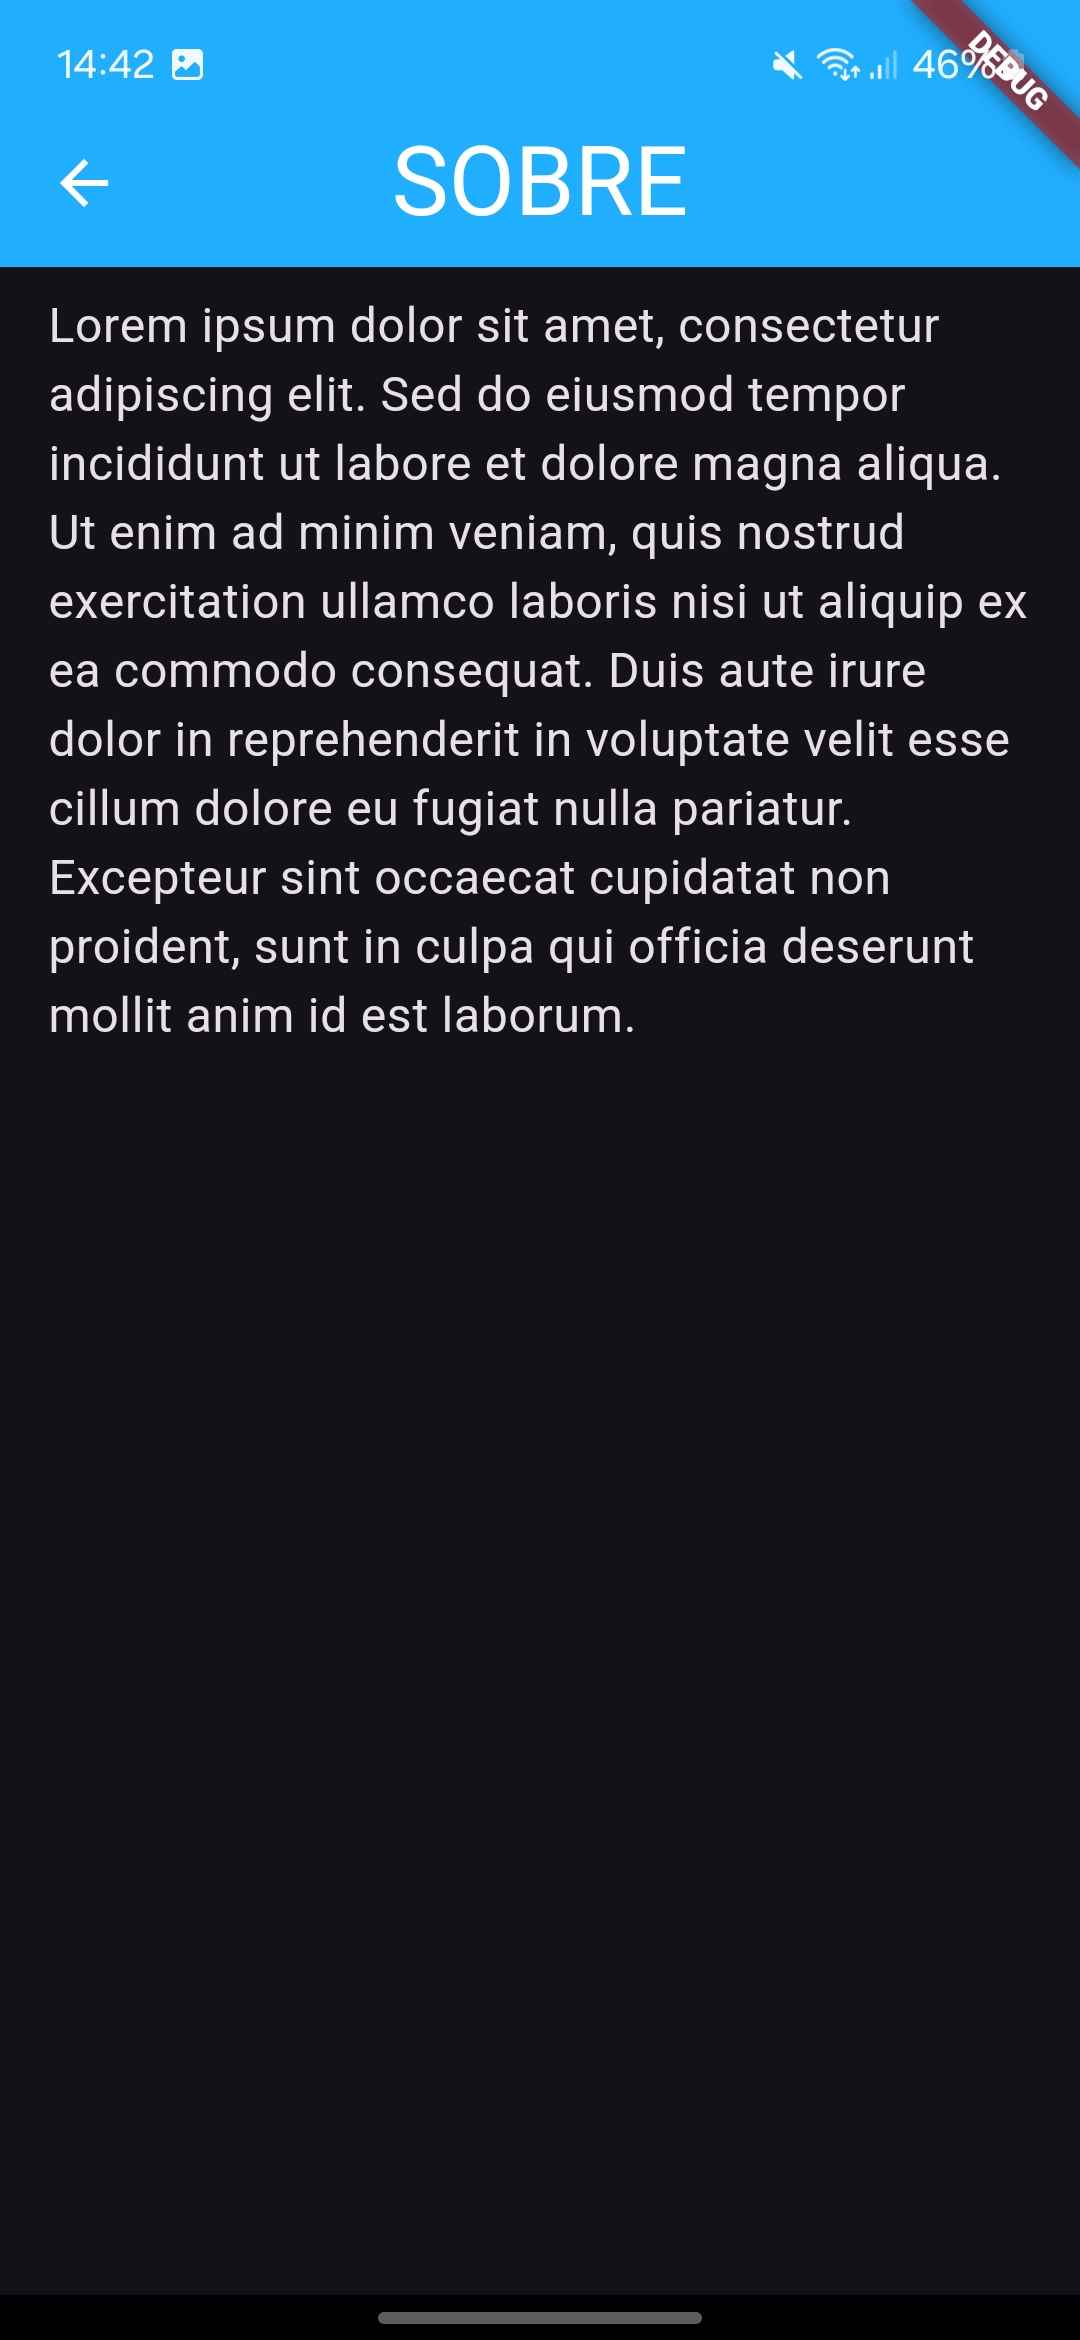
\includegraphics[width=0.4\textwidth]{imagens/sobre.jpg}
        \caption{\scriptsize Tela 6: Sobre}
        \label{fig:tela6}
    \end{figure}

    \FloatBarrier

\subsubsection{Tela 7: Login}

    A tela de login pode ser alcançada através de 2 fluxos, o primeiro é através do botão de Login na tela de Menu Lateral e o segundo é quando o usuário tentar marcar um local como favorito sem estar logado. A tela de login é composta por um campo de e-mail e um campo de senha, além de botões para iniciar o processo de registro de uma nova conta ou para recuperar a senha, caso o usuário tenha esquecido. A Figura 15 mostra a tela de login e de cadastro.

    \begin{figure}[h]
        \centering
        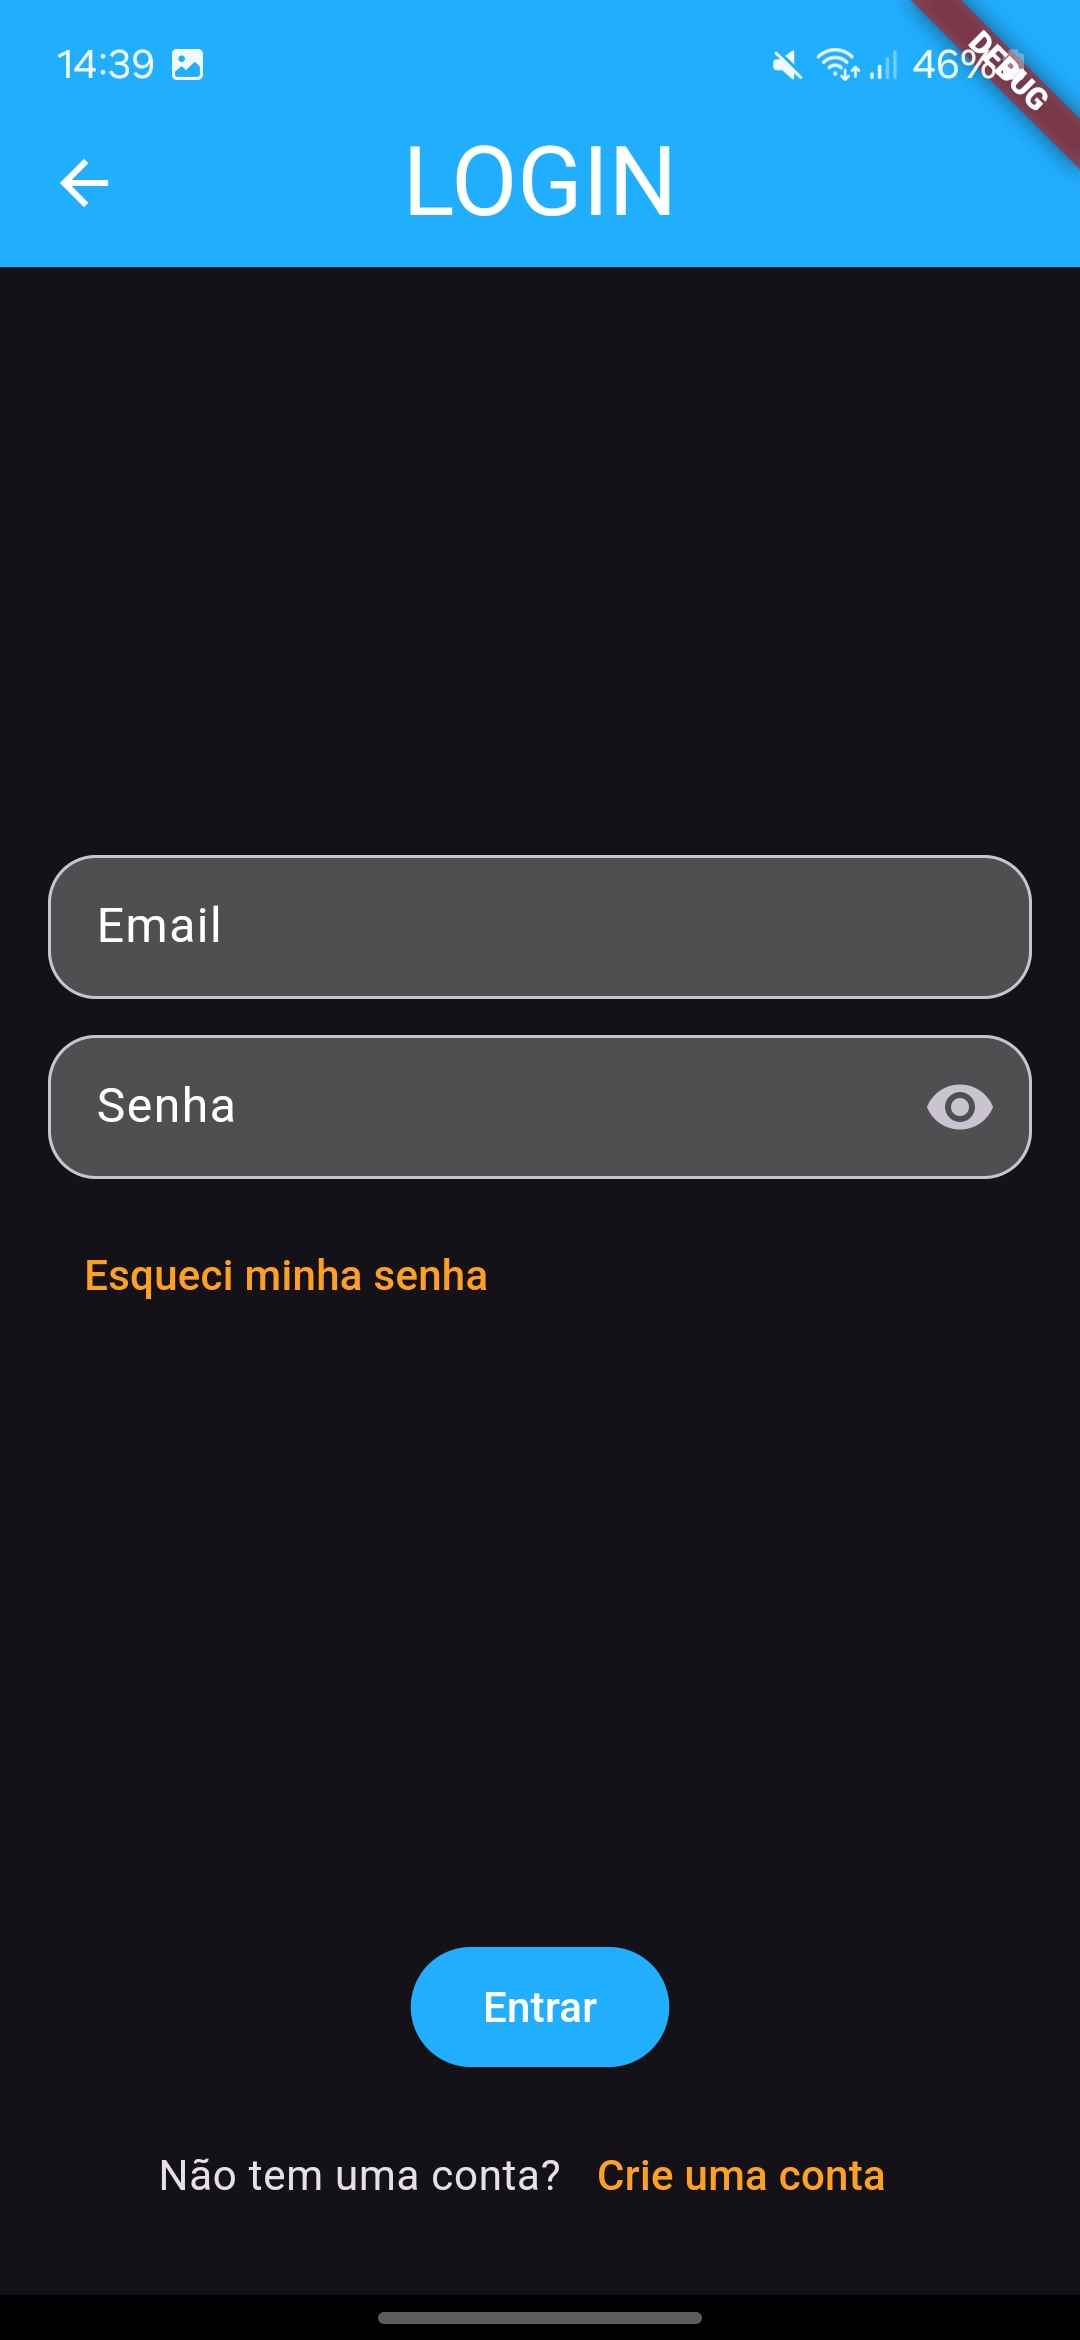
\includegraphics[width=0.4\textwidth]{imagens/login.jpg}
        \hspace{10mm}
        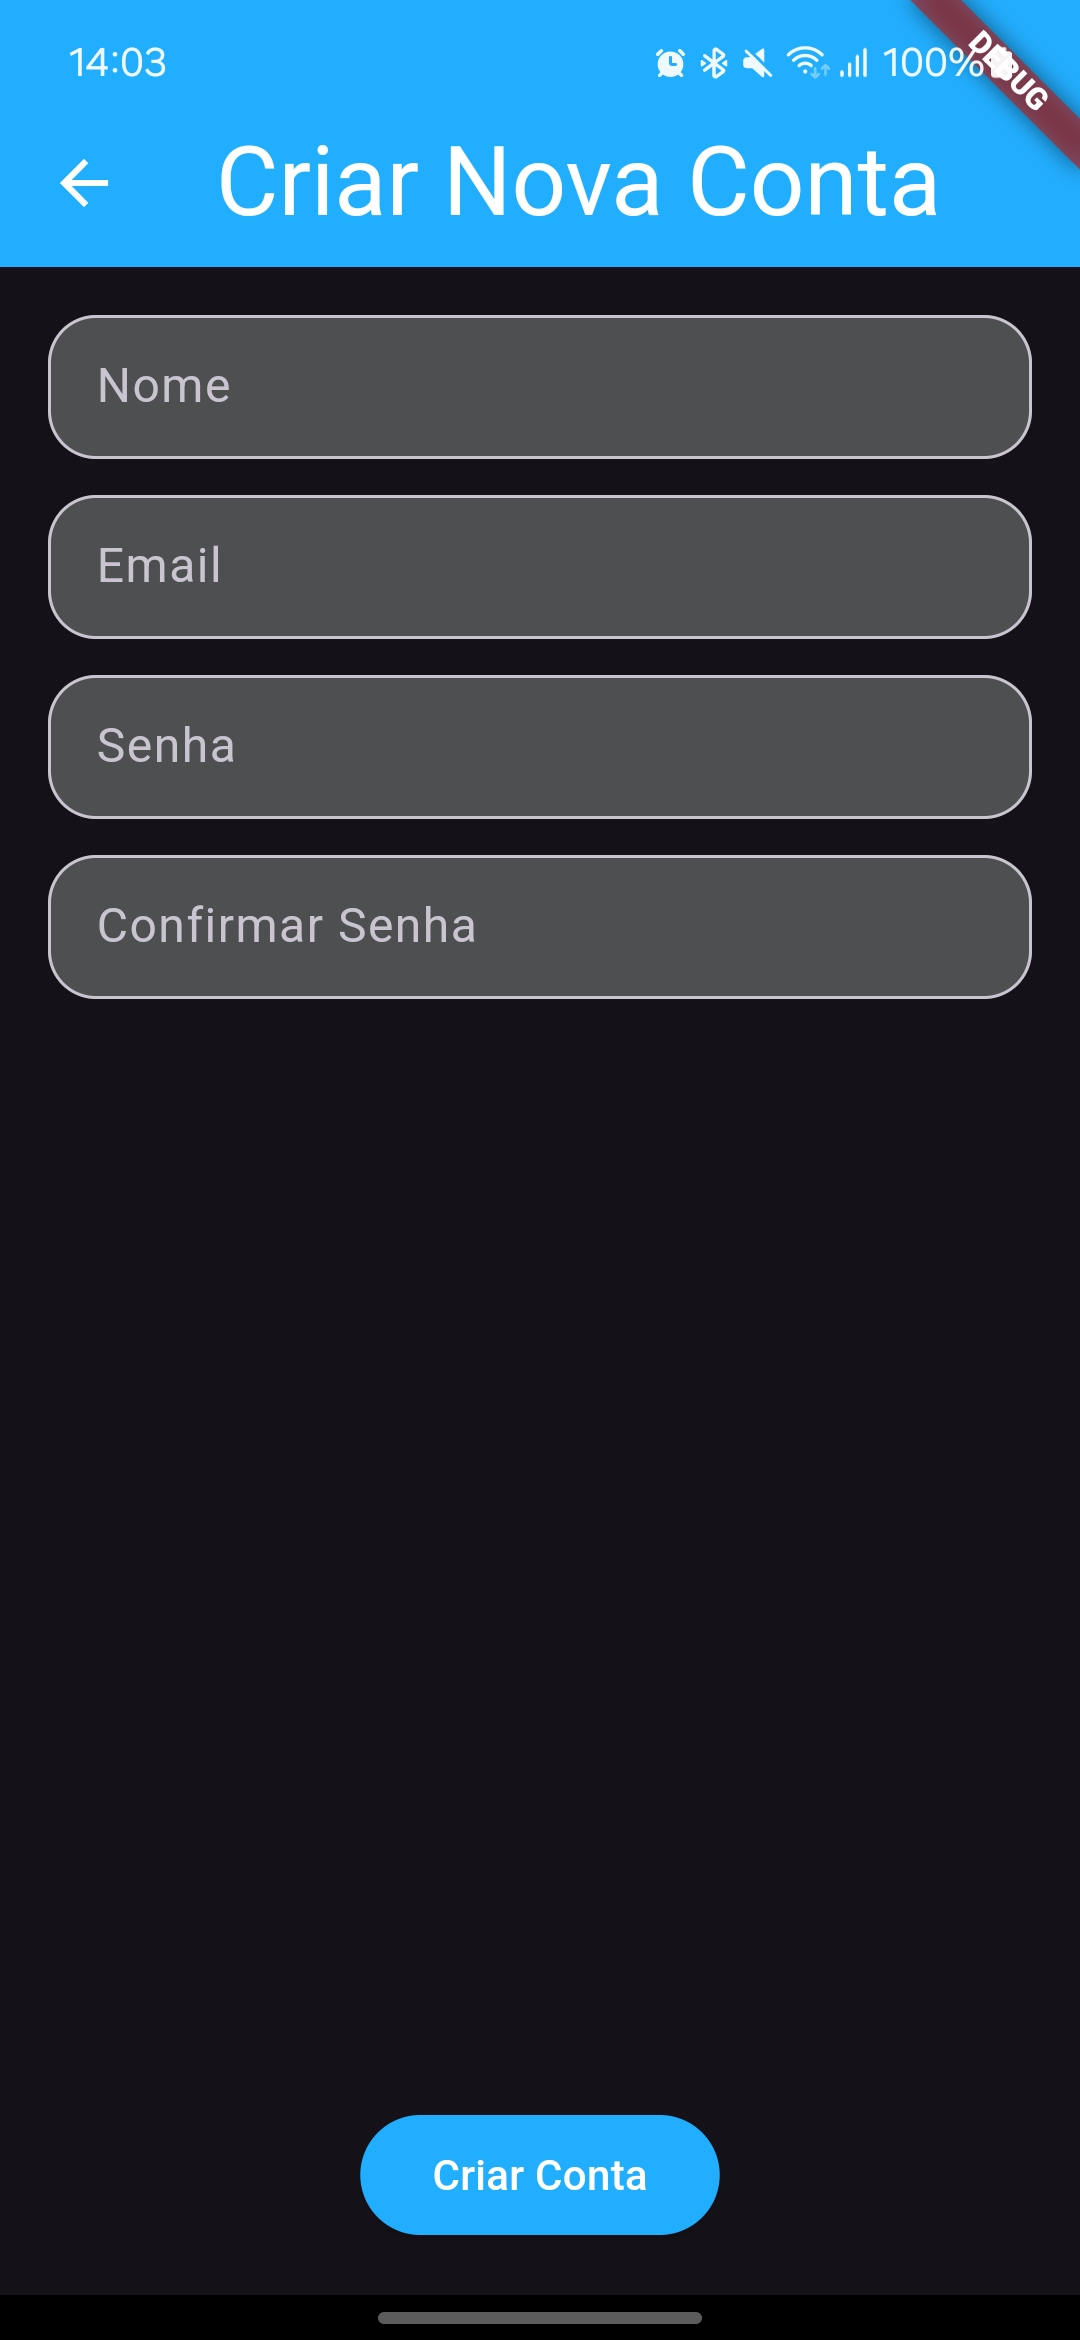
\includegraphics[width=0.4\textwidth]{imagens/registrar.jpg} %tela de registro
        \caption{\scriptsize Tela 7: Login}
        \label{fig:tela7}
    \end{figure}

    \FloatBarrier
    
    Caso o usuário entre no processo de recuperação de senha ele deverá informar o email cadastrado e um email será enviado com um código de recuperação, que deverá ser informado numa tela subsequente, caso a verificação seja bem sucedida o usuário poderá definir uma nova senha. A Figura 16 mostra as telas de recuperação de senha.
    
    \FloatBarrier

    \begin{figure}[h]
        \centering
        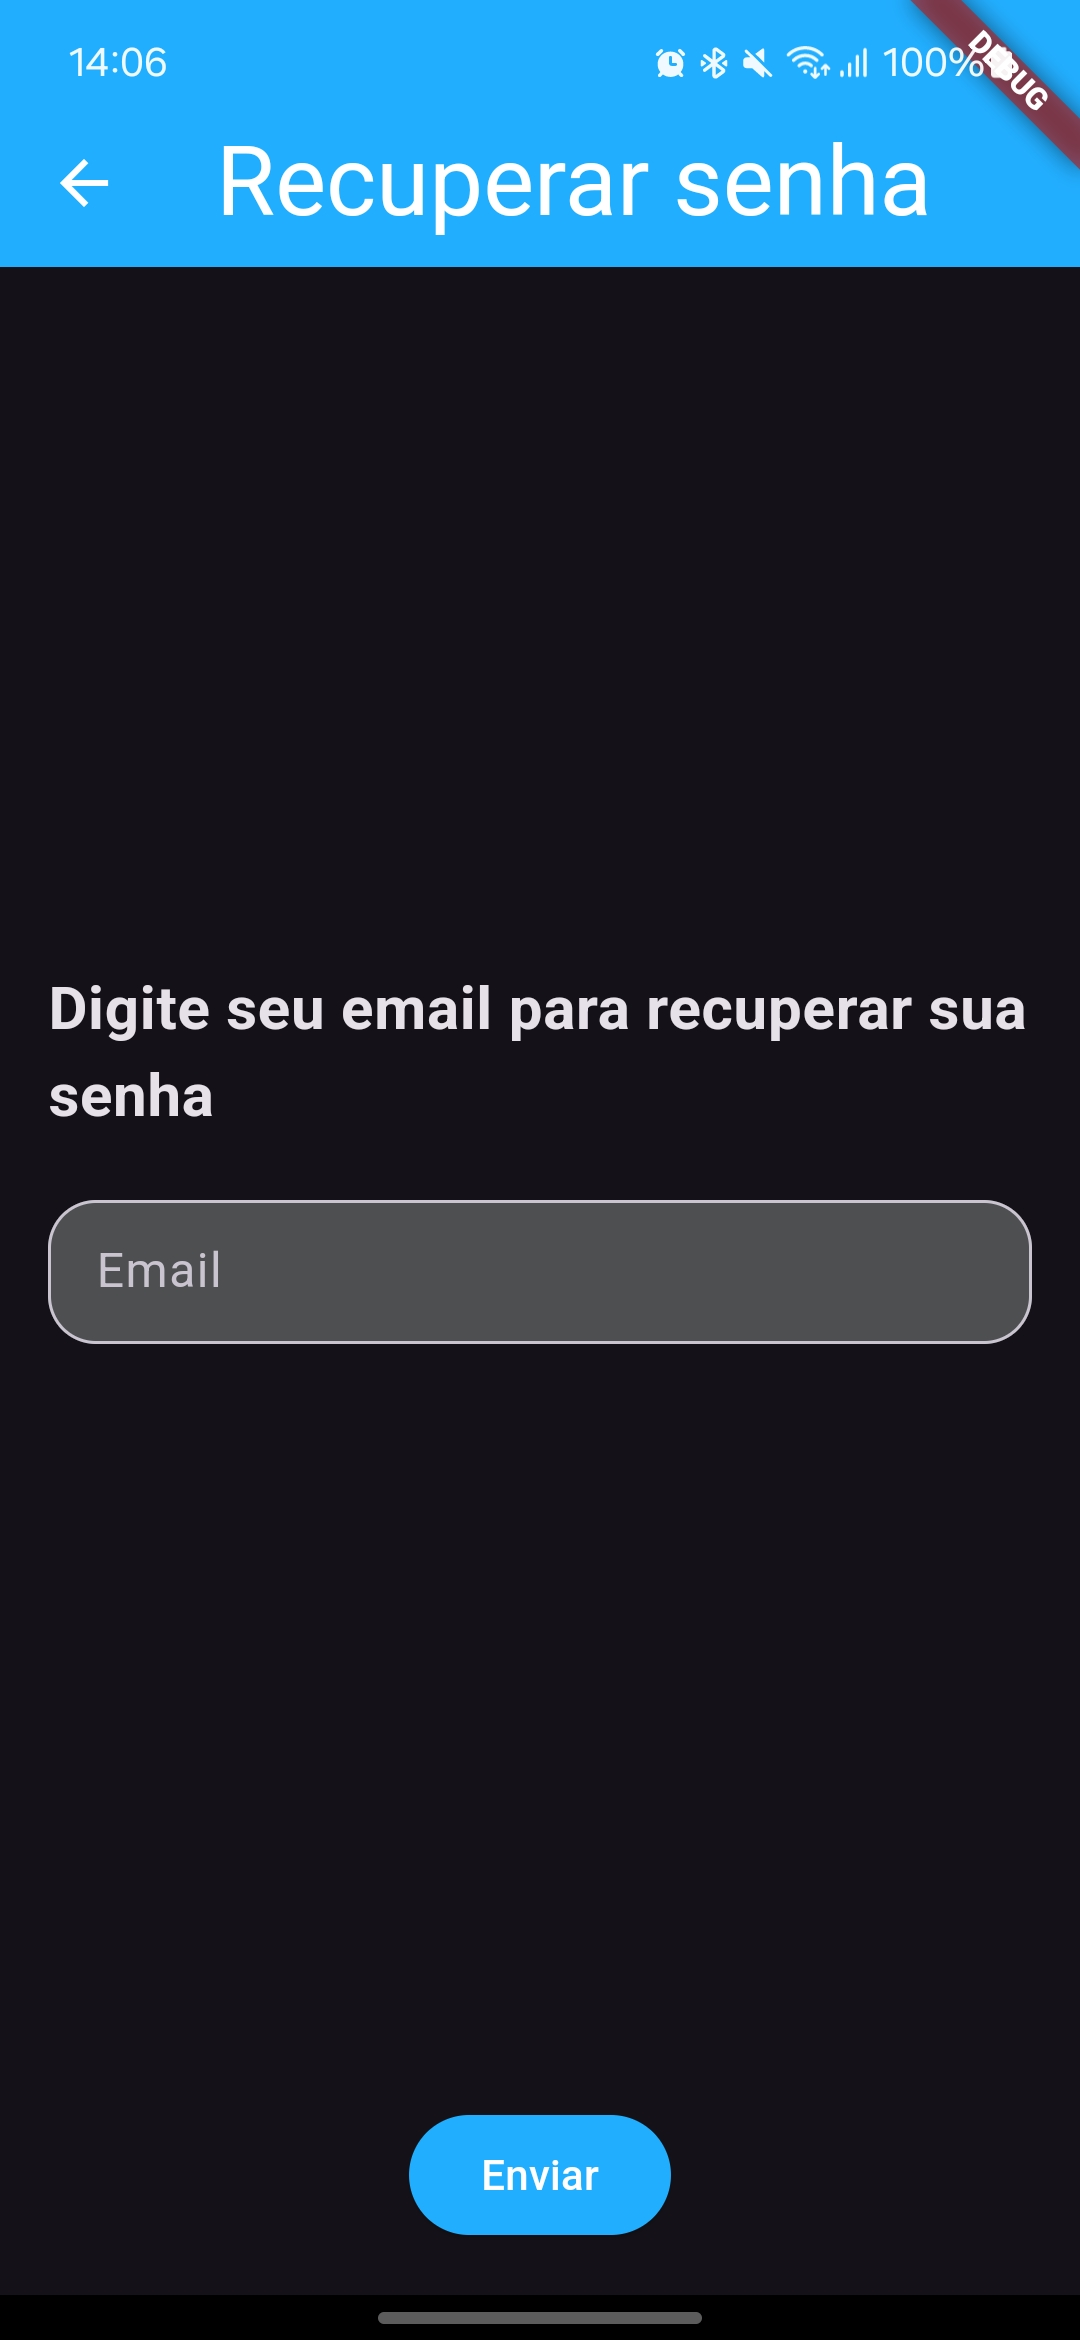
\includegraphics[width=0.4\textwidth]{imagens/email.jpg} %tela de email
        \hspace{10mm}
        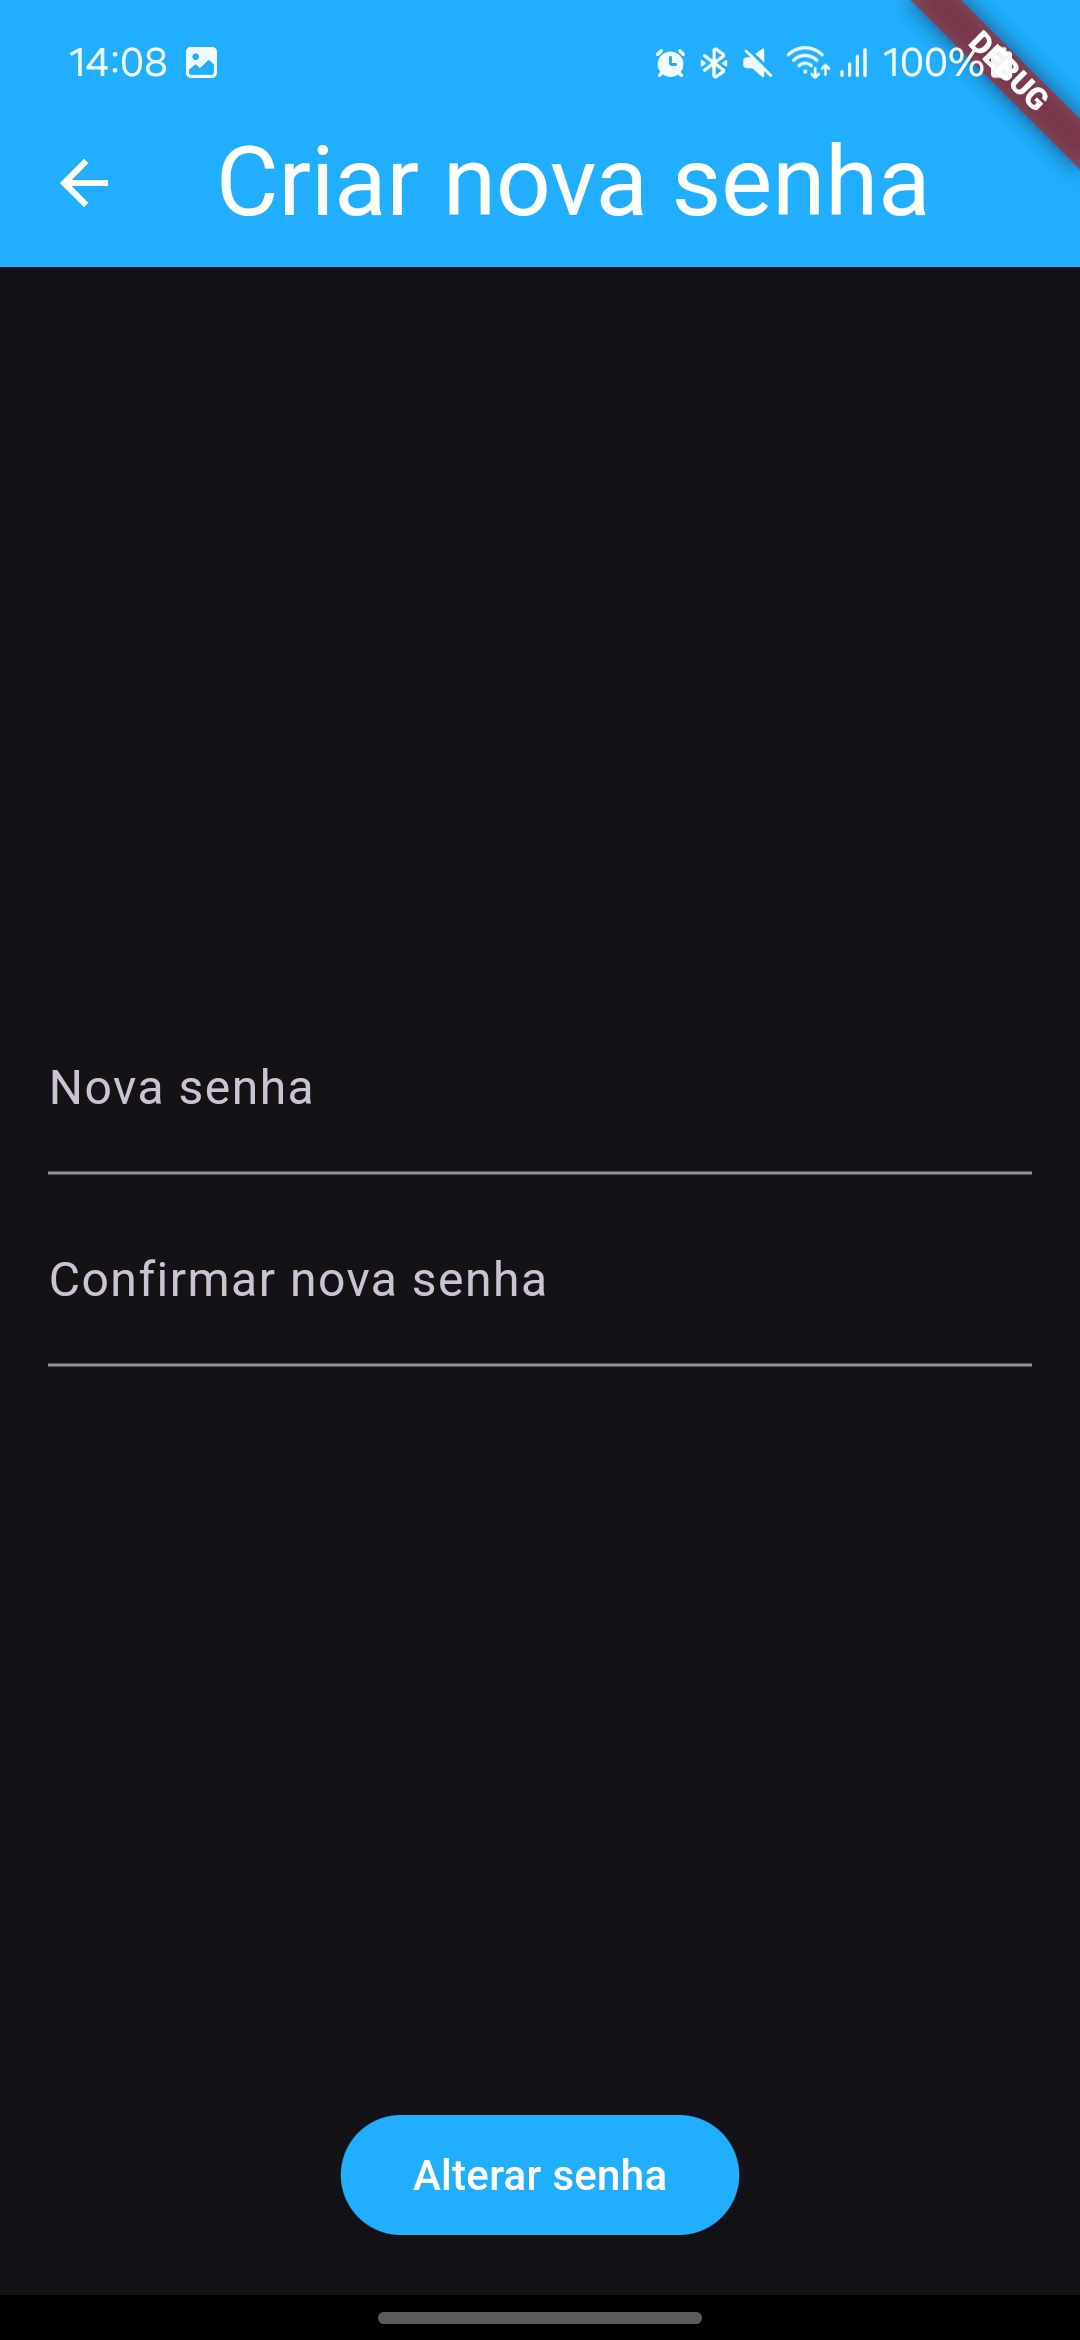
\includegraphics[width=0.4\textwidth]{imagens/nova-senha.jpg} %tela de codigo
        \caption{\scriptsize Tela 7: Login}
        \label{fig:tela7-recuperacao}
    \end{figure}

    \FloatBarrier

\section{Considerações Finais}

\section{Trabalhos Futuros}
\label{sec:trabalhos_futuros}

    Por mais que o aplicativo já seja funcional, vemos que ainda há muito espaço para melhorias e novas funcionalidades. A seguir, listamos algumas ideias para trabalhos futuros:
    
    Requisitos que foram levantados mas não implementados seriam um bom ponto de partida para futuras implementações. Alguns exemplos são a possibilidade de se registrar e entrar no aplicativo através de serviços externos como o Google e o Facebook, o histórico de pesquisa para facilitar a experiência do usuário, a introdução de um modo claro e a adição de opções de acessibilidade mais avançadas.
    
    Seria interessante adicionar uma seção de comentários nos locais, onde os usuários pudessem deixar suas opiniões e avaliações mais detalhadas sobre o funcionamento do local. Isso poderia para serviços como o de restaurantes e lanchonetes, por exemplo.

    Essas melhorias fariam o Encontre na UFMS mais completo e agradável de se usar, o que consolidaria seu uso e popularidade entre os estudantes e visitantes da UFMS.

\FloatBarrier

\bibliographystyle{plain}
\bibliography{referencias}
\label{sec:referencias}

\end{document}
